\documentclass{report}

% Language setting
% Replace `english' with e.g. `spanish' to change the document language
\usepackage[english]{babel}

% Set page size and margins
% Replace `letterpaper' with `a4paper' for UK/EU standard size
\usepackage[letterpaper,top=2cm,bottom=2cm,left=3cm,right=3cm,marginparwidth=1.75cm]{geometry}

% Useful packages
\usepackage{amsmath}
\usepackage{graphicx}
\usepackage{float}
\usepackage{subcaption}
\usepackage{chronology}
\usepackage{listings}

\usepackage[colorlinks=true, allcolors=blue]{hyperref}

\newtheorem{definition}{Definition}[section]

\title{Interim Report}
\author{Vinay Kakkar}

\begin{document}
\maketitle

\tableofcontents

\begin{abstract}
    Currently, biologists are analysing PDB files that contain structural protein data in which they can determine something from running a user executable on to it. Biologists can determine many things from the analysis of these types of data. Biologists are then able to aid in new drug discoveries as a result help create new medicine for mutated proteins that might not be in living cells at the moment. This project aims to help that process in being able to gather lots of data together and make it efficient for a biologist to run an executable onto these files. To do this I delve into protein structures in the PDB bank and Hadoop/spark which provides batch processing features that allow me to distribute these files onto a cluster that is then able to run in parallel. This is my interim report in which I explain my proof of concept programs to show that this framework is possible and will help the structural bioinformatics department in analysing thousands of data in a very quick manner.

\end{abstract}

\renewcommand\thesection{\arabic{section}}

\section{Aims, objectives and Literature Survey}

\subsection{Aims}
\subsubsection{Aim provided in the Project description} 

Provide a framework where large numbers of protein structures can be analysed using a user-provided executable in the MapReduce formalism.

\subsubsection{Aim in more depth}
When a biologist conducts analysis on a protein structure they can learn about the functionality and behaviour of the protein. With this aim it is very beneficial for the biology sector as this will help them perform large scale data analysis on to protein structures. This is very helpful as it allows biologists to be able to learn from the analysis about protein structures functionality and behaviours in a more efficient manor. As a result, this will allow biologists to be able to create a new drug which can help with future or current diseases called new drug discovery. 

By using batch processing and large-scale data processing will give the biologist the ability to do so. This means that given lots of protein structures the user would be able to pass each protein structure of their choice into a executable of their choice that will return a result. As a result, being able to perform more analysis on more protein structures yielding faster results. More specifically we can use Hadoop or Spark with python to store these protein data and process the data in parallel so that multiple proteins can be processed at the same time giving better speeds and performance yielding faster results.

For this to be possible we need to build a program that functions as a framework that has multiple user executables and that can be flexible in adding in newer created executables in the future which can be picked by the user when deciding what analysis, they want to conduct. essentially this program should be able to handle the protein data provided by the protein data bank and most the file types provided by it. It is important that the user should be able to choose what protein data it wants to send into the framework and what executable they want to conduct on these files.

\subsection{Objectives}

To achieve the aims provided in section 1 i will need to complete a set of objectives which once finished will suggest that the aim has be met and that I fulfil the needs for the aims.

\subsubsection{ObjectivesCompleted}

\subsubsection{Tutorials}

In order to complete the projects aim i need to understand some technologies:

\begin{itemize}
    \item Spark
    \item Pythons API for Spark pyspark
    \item How to create a cluster
    \item How to perform Mapreduce
    \item How to set up a local cluster
\end{itemize}

I went through a few tutorials which are named in my readme file within GitLab.

The first two tutorials showed me how to set up pyspark and how to use spark and python together. This was mainly to do with the setup and basics of spark.

The next tutorial taught me how to conduct MapReduce within pyspark on spark dataframes. Focusing more on complicated features such as MapReduce functions of spark and how they work.

Lastly, the last tutorial showed me how to distribute these dataframes on a cluster (local) by turning the dataframes into an RDD which can be spread across the nodes of a cluster.

 I tried to follow a tutorial that showed me the basics of setting up a cluster among computers but this quickly escalated and did not fit within the time frame and schedule I had planned.

\subsubsection{Proof of Concept}

Before beginning my program I try to achieve the needs of my aim. To do this I need to create a program that proves that it is possible. The two main things I need to prove are that I can set up a cluster and distribute a single file amongst it. It is important to note I use the correct file type which will relate to the same type I would use in the actual program. The second thing I need to prove is that I can run a simple executable onto this file which is distributed. As if I can do both features then it shows that my actual program will indeed work and I wont run into any unfixable blocks along the way.

\subsubsection{Distributing Protein Structure Files Amongst MapReduce cluster}

First action to take is create a local cluster. Then we need to read a .pdb file or multiple in a directory and convert it into a spark dataframe which is then converted into a rdd so that it can be distributed on to the nodes in the cluster(in this case it will be how every many cores i give my local cluster).

\subsubsection{Running MapReduce using a single type of executable for Analysing Protein Structures}

This is completed by collecting all the data from an rdd back into dataframes and then pack each datafram value into a PDB file which we can then run user executables on to yield a result.


\subsubsection{Reports}

Whilst working on the proof of concept programs I also need to research the data I am going to be working with.

\subsubsection{Protein Structures}

Researching this topic gave me in-depth knowledge of protein structures and large-scale expressions for example different methods used on how the data is extracted to be fed into the file. This gave me insight into the files I am working with and also aided me to navigate through the PDB website as I understood some of the hard biological language used within the site.

\subsubsection{The Protein Data Bank and the file formats}

The protein data bank provides the data in fields that can be of three different types; .pdb, .mmcif, .XML


This is important as it will be the file types I will be working with for example I will need to put some of these file types into a cluster whilst working with pyspark. This gave me insight into how to read these files and made it easier to create my proof of concept programs as I understood results when trying to read the file or turning the file into a dataframe.

\subsection{Futher Objectives}

The Objectives provided above are completed but together do not satisfy the needs of the aims there are some objectives left that i will need to complete to complete each aim listed these include:

\begin{itemize}
    \item Provide some form of UI so that a user can pick what executables to perform and also be able to upload what protein structures they want to provide analysis on.
    \item Be able to perform/use user executables that are perfomred on pdb files which will yeild a result (Currently my proof of concept program runs a terminal command that returns the number of lines present in the .pdb file).
    \item Reasearch on how to distribute clusters to multiple computers allowing them to comunicate and perform actions and achive goals needed by working together.
    \item Reasearch on how to conduct benchmarking comparing the speeds difference when trying to accomplish the same task but not using batch processing.
    \item Provide a clear set of guidelines for the map/reduce executables.
\end{itemize}

These objectives will form the basis for my second term work and so will my time scale be created from these.


\subsubsection{Extensions}

If given the change/time i would work on some extra features that will improve my program. Some extensions i have thought of are:

\begin{itemize}
    \item Use a very big data set as a test. For example, this data set can be a subset mirror of the pdb site. This can yield intresting results in testing the performance of my framework.
    \item Improved ui as biologists are not to deep in the computer science sector having a easy ui can really help and enahnce there experiance whilst using this program.
    \item A set of user executables that are ready and just need to be selected by the user.
    \item Implementation on a Public Mapreduce cluster e.g. Amazon.
\end{itemize}


\section*{literature survey}

\section{Protein Structures}

\subsection{Introduction}

Amino acids are molecules that when combined forms proteins. All of the 20 amino acids, see table~\ref{Amino acids} have in common a central carbon atom which is attached to a hydrogen atom, an amino group, and a carboxyl group. What distinguishes one amino acid from another is the side chain attached to the central carbon atom through its fourth valence~\cite{branden_introduction_1998}.

\begin{table}[h!]
    \begin{center}
    \label{tab:Amino acids}
        \begin{tabular}{l|c|r}
        Amino acid & Three-letter code & One-letter code\\
        \hline
        \\
        Glycine & Gly & G\\
        Alanine & Ala & A\\
        Valine & Val & V\\
        Leucine & Leu & L\\
        Isoleucine & Ile & I\\
        Proline & Pro & P\\
        Phenylalanine & Phe & F\\
        Methionine & Met & M\\
        Tryptophan & Trp & W\\
        Cysteine & Cys & C\\
        \\
        \hline
        \\
        Asparagine & Asn & N\\
        Glutamine & Gln & Q\\
        Serine & Ser & S\\
        Threonine & Thr & T\\
        Tyrosine & Tyr & Y\\
        \\
        \hline
        \\
        Aspartic acid & Asp & D\\
        Glutamic acid & Glu & E\\
        \\
        \hline
        \\
        Histidine & His & H\\
        Lysine & Lys & K\\
        Arginine & Arg & R\\
        \end{tabular}
        \caption{\label{Amino acids}The 20 amino acids. The amino acid name, the three-letter code, and the one-letter code are given. The Amino acids are split up into Nonpolar, Polar, Acidic and Basic respectfully}
    \end{center}
\end{table}

Proteins are responsible for catalysing most of the chemical reactions in cells. They can function as enzymes catalysing a wide variety of reactions important for life and thus also important for the structure of living systems such as proteins involved in the cytoskeleton. The size of protein can vary ~\cite{zvelebil_understanding_2008}.

\begin{definition}[Catalysing]
    Catalysing is to make a chemical reaction happen or happen more quickly by acting as a catalyst.
\end{definition}

\begin{definition}[Cytoskeleton]
    A dynamic network of interlinking protein filaments present in the cytoplasm of all cells~\cite{zvelebil_understanding_2008}. 
\end{definition}

We can analyse a DNA sequence of a gene to retrieve the amino acid sequence of the protein product, using the fact that proteins are built up of amino acids. Leaving a position where we can help deduce the likely properties of unknown proteins, whilst at the same time including their functions and structures. Knowing the relationship between a protein's structure and its function provides a better understanding of how the protein works with better understand this we can conduct experiments to explore how modifying the structure will affect the function. The use of bioinformatics aids this process whilst also providing computer modeling for these interactions~\cite{zvelebil_understanding_2008}.

\subsection{Primary, Secondary, Tertiary and Quaternary Structure}

Please refer to~\ref{fig:levels of protein structure.} for a visual representation.

\subsubsection{Primary Structure}

The primary structure of a peptide or protein is the linear sequence of its amino acids. It is read and written from the amino-terminal to the carboxyl-terminal end. Where each amino acid is connected to the next by a peptide bond. Primary structure sequence it can interact with one another to form secondary structures~\cite{sun_overview_2004}.

\subsubsection{Secondary Structure}

The secondary structure refers to the local arrangement of a peptide chain. Where several common secondary structures have been identified in proteins~\cite{sun_overview_2004}.

\subsubsection{Tertiary Structure}

Tertiary structure is a three-dimensional structure of a protein the formation is built up of bonds and interactions that serve to change the shape of the overall protein. Finaly the folding that we end up with for a given polypeptide is the tertiary structure~\cite{godbey_chapter_2022}.

\subsubsection{Quaternary Structure}

The quaternary structure of a protein is built-up of several protein chains/subunits. Each of the subunits has its primary, secondary, and tertiary structure. The subunits are held together by hydrogen bonds and van der Waals forces between nonpolar side chains~\cite{ouellette_14_2015}. I highlighted some proteins with Quaternary structures~\ref{Quanternanry Protiens}.

\begin{definition}[Van Der Waals]
    A relatively weak electric force attracts neutral molecules that collide with or pass very close to each other~\cite{noauthor_210_2018}.
\end{definition}

\begin{table}[h!]
    \begin{center}
    \label{tab:Quanternanry Protiens}
        \begin{tabular}{l|c|r}
            \hline
            Protein & Number of Subunits & Function\\
            \hline
            Alcohol dehydrogenase & 4 & Enzymatic reaction in fermentation\\ 
            \hline
            Aldolase & 4 & Enzymatic reaction in glycolysis\\
            \hline
            Fumarase & 4 & Enzymatic reaction in citric acid cycle \\
            \hline
            Hemoglobin & 14 & Oxygen transport in blood\\
            \hline
            Insulin & 2 & 6344\\
            \hline
        \end{tabular}
        \caption{\label{Quanternanry Protiens}Examples of Proteins Having Quaternary Structure~\cite{ouellette_14_2015}.}
    \end{center}
\end{table}

\begin{figure}[H]
    \centering
    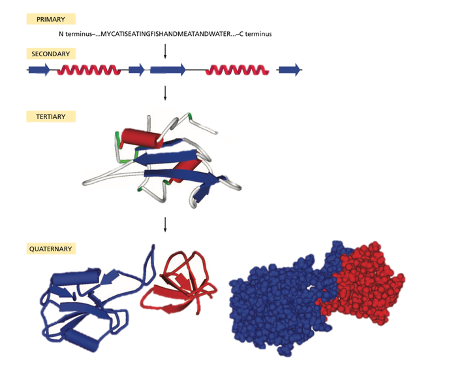
\includegraphics[width=0.5\textwidth]{Protein Structure.png}
    \caption{\label{fig:levels of protein structure.}From the sequence alone, the primary structure to secondary structure, to tertiary structure(3D), to finally quaternary structure found when several tertiary structures form a multisubunit complex~\cite{zvelebil_understanding_2008}.}
\end{figure}


\subsubsection{Considering Protein structure on several different levels}

The fold of the protein plays part in determining the way the protein will function, and also whether it will function correctly so it is important to understand these folds refer to~\ref{fig:levels of protein structure.} to see what a protein fold looks like. Which we can use to help us for example predict the fold of a protein from its sequence. Looking at Protein structures on different levels we need to consider the analysis of protein structure by experimental techniques such as X-ray crystallography, nuclear magnetic resonance, and RNAseq which show that proteins adopt distinct structural elements~\cite{zvelebil_understanding_2008}.

\subsubsection{Amino Acids}

When looking at a primary structure of a protein~\ref{fig:levels of protein structure.} the sequence of amino acids~\ref{Amino acids} will build up the linear protein chain. This linear chain is often called a polypeptide chain~\cite{zvelebil_understanding_2008}.

Amino acids are different from each other due to their side chains and due to this the functional properties of various different proteins are different. Each type of amino acid has specific chemical-physical properties determined by the structure and chemical properties of its side chain. They can, however, be classified into overlapping groups that share some common physical and chemical properties~\cite{zvelebil_understanding_2008}. You can see the amino acids grouped here~\ref{Amino acids}.

\begin{figure}[H]
    \centering
    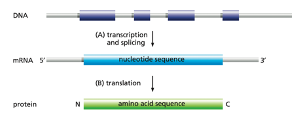
\includegraphics[width=0.5\textwidth]{Transcription and translation.png}
    \caption{\label{fig:Transcription and translation}The relation of DNA coding-strand sequence to mRNA sequence to protein sequence. The exons of the DNA are transcribed into mRNA which, using other molecules directs the protein sequence~\cite{zvelebil_understanding_2008}.}
\end{figure}

\subsubsection{Bioinformatic Difficulties with Predictions on Proteins}

It is difficult to define the precise ends of the helices(The secondary structure of proteins is made up of a-helices and b-strands) for structures found in globular proteins that are not perfectly regular. Making it one step more difficult when trying to predict these structures~\cite{zvelebil_understanding_2008}.

To Note:
\begin{itemize}
    \item Several different types of b-sheet are found in protein structures.
    \item Turns, hairpins, and loops connect helices and strands. 
    \item Any chain between two regular structures is referred to as a loop.
    \item Mostly a loop will contain a turn (or even several).
\end{itemize} 

In antibody recognition, immunoglobulins employ loops at the edge of a b-sheet. All immunoglobulin structures with the same overall chain fold, but it is the difference at these loops that results in different results. Loops take up one of a limited number of structures called canonical forms. This type of classification is another reason why trying to predict both the structure and function of the protein is difficult~\cite{zvelebil_understanding_2008}.

\begin{definition}[Immunoglobulin]
    Immunoglobulins are heterodimeric proteins composed of two heavy and two light chains. Types of white blood cells that helps the body fight infection~\cite{schroeder_structure_2010}.
\end{definition}

\subsection{Large Scale Experssion}

Gene expression begins when genes are transcribed into messenger RNAs, which are then translated to produce proteins. 

Total gene expression in cultured cells or a tissue sample can be detected in three main ways:

\begin{enumerate}
    \item DNA microarray technology.
    \item Two-dimensional Gel electrophoresis or Chromatography.
    \item RNAseq
\end{enumerate}

With the first two cases, they produce enormous amounts of raw data~\cite{zvelebil_understanding_2008} due to this, many proteins currently evade high-resolution structure determination. Structural mass spectrometry is a powerful approach that is better than the first two methods mentioned above, by having nearly an unlimited size constraint and speed. Although the data provided by mass spectrometry is vague for full high-resolution structure elucidation, structural mass spectrometry can be used to examine the size, solvent accessibility, and topography of proteins~\cite{limpikirati_covalent_2018}~\cite{liu_mass_2020}.  Many mass spectrometry techniques exist that can elucidate elements of protein tertiary and quaternary structure~\cite{biehn_protein_2022}.

We can have computational methods that aid experimental technique intending to elucidate protein structures~\cite{seffernick_hybrid_2020}~\cite{leman_macromolecular_2020}. Software packages can be used to combine data with advanced structure sampling and scoring techniques. Computational tools for protein structure modeling, include the Rosetta software suite~\cite{leman_macromolecular_2020}~\cite{alford_rosetta_2017}, I-TASSER~\cite{yang_i-tasser_2015}, Phyre2~\cite{kelley_phyre2_2015}, Integrative Modeling Platform~\cite{russel_putting_2012}, HADDOCK~\cite{dominguez_haddock_2003}, and MODELLER~\cite{eswar_comparative_2006}~\cite{biehn_protein_2022}.

\subsubsection{Large Scale Gene Expression}

Genome DNA microarray experiments produce large amount of data can be computationaly heavy on where methods can yield alternative conclusions from inceasing the computational effort.

The goal of these experiments is to determine biological or functional meaning from the lists of genes, either by:

\begin{enumerate}
    \item Identify critical genes that are responsible for a biological effect.
    \item Find patterns within the genes that point to an underlying biological process.
\end{enumerate}
\cite{zvelebil_understanding_2008}

\begin{figure}[H]
    \centering
    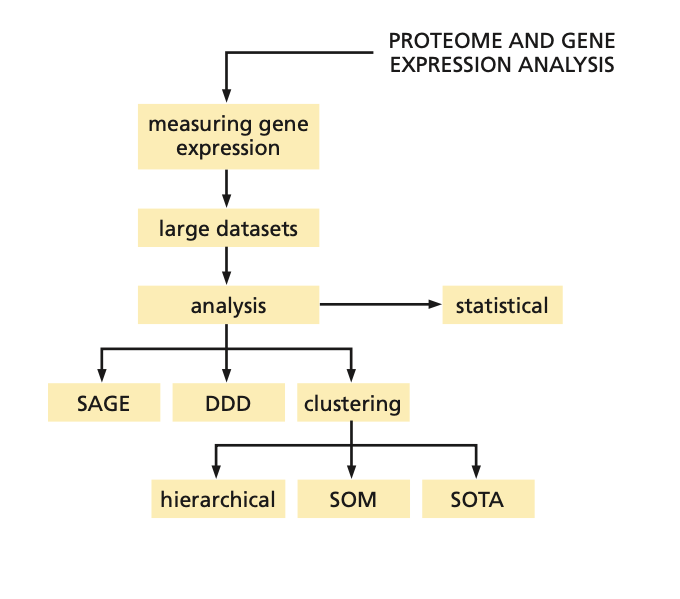
\includegraphics[width=0.5\textwidth]{Gene Expresion.png}
    \caption{\label{fig:Gene Expression}Describing Common experimental aspects of gene expression and of the analysis of the resulting data~\cite{zvelebil_understanding_2008}.}
\end{figure}

\subsubsection{Serial analysis of gene expression}

Serial analysis of gene expression is the alternative compared to microarrays when trying to investigate patterns of gene expression.

\begin{figure}[!h]
    \centering
    \begin{subfigure}[t]{.45\textwidth}
        \centering
        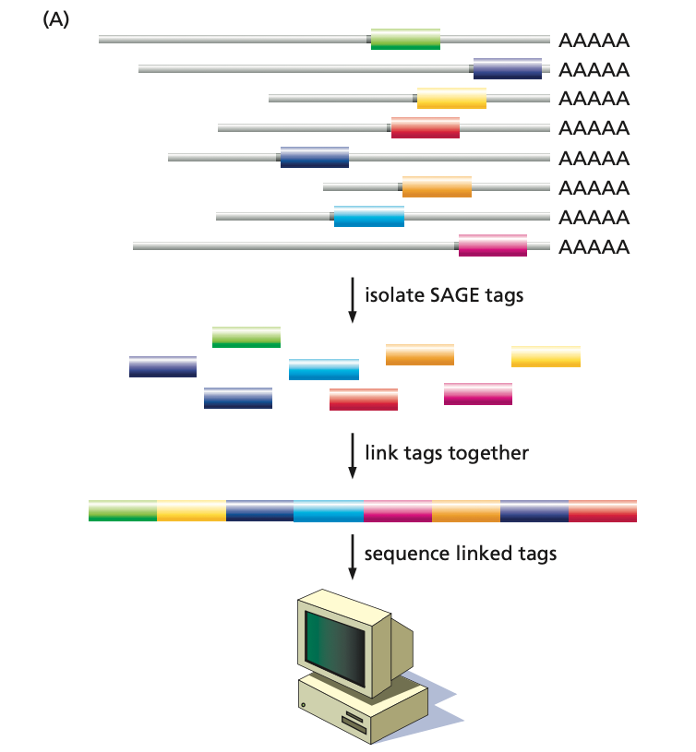
\includegraphics[width=0.9\textwidth]{SAGE1.png}
        \caption{}
        \label{fig:SAGE1} 
    \end{subfigure}
    \begin{subfigure}[t]{.45\textwidth}
       \centering
       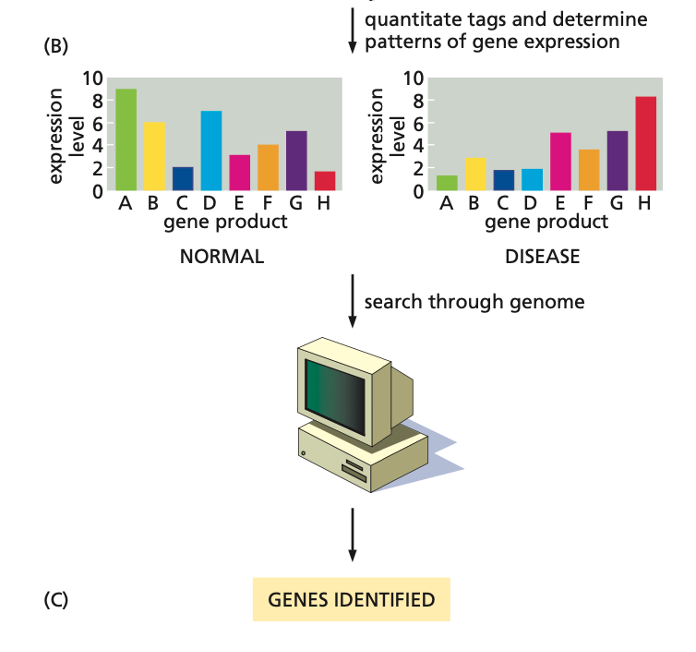
\includegraphics[width=0.9\textwidth]{SAGE2.png}
       \caption{}
       \label{fig:SAGE2}
    \end{subfigure}
    \caption{\emph{An outline of the SAGE method for comparing levels of gene expression. (A) Short sequence tags. The sequence tags are isolated and are linked together to produce long DNA molecules that can be cloned and sequenced. (B) Once sequenced, each tag can be calculated, resulting in a value that gives the expression level of the corresponding transcript~\cite{zvelebil_understanding_2008}.}}
    \label{fig:SAGE}
\end{figure}

A short sequence contains enough information to uniquely identify a gene. The sequence tags from the total cellular RNA can be linked together to form long DNA molecules. The total number of times a particular tag is observed the concatemers approximates the expression level of the corresponding gene. The data produced by SAGE include a list of the tags with their corresponding counts, providing a digital output of cellular gene expression.  Which allows the user to specify which organ is to be investigated. Libraries consisting of gene lists organized by the various types of tissues or cell lines are provided for further choice. The output from SAGE provides the SAGE tag, the UniGene ID, the gene description, and color and letter-coded differences in expression levels~\cite{zvelebil_understanding_2008}.

\subsubsection{Clustered gene expression data}

Clustered pattern data obtained from gene expression microarrays/genome bioinformatics can be used as a tool to identify new transcription factors or other cell-regulatory proteins. 

The clustered genes/proteins can be analyzed. Leading to a vast collection of data from many gene/protein expression experiments being available on the Web~\cite{zvelebil_understanding_2008}.

\subsubsection{Large Scale Protein Expression}

\begin{figure}[H]
    \centering
    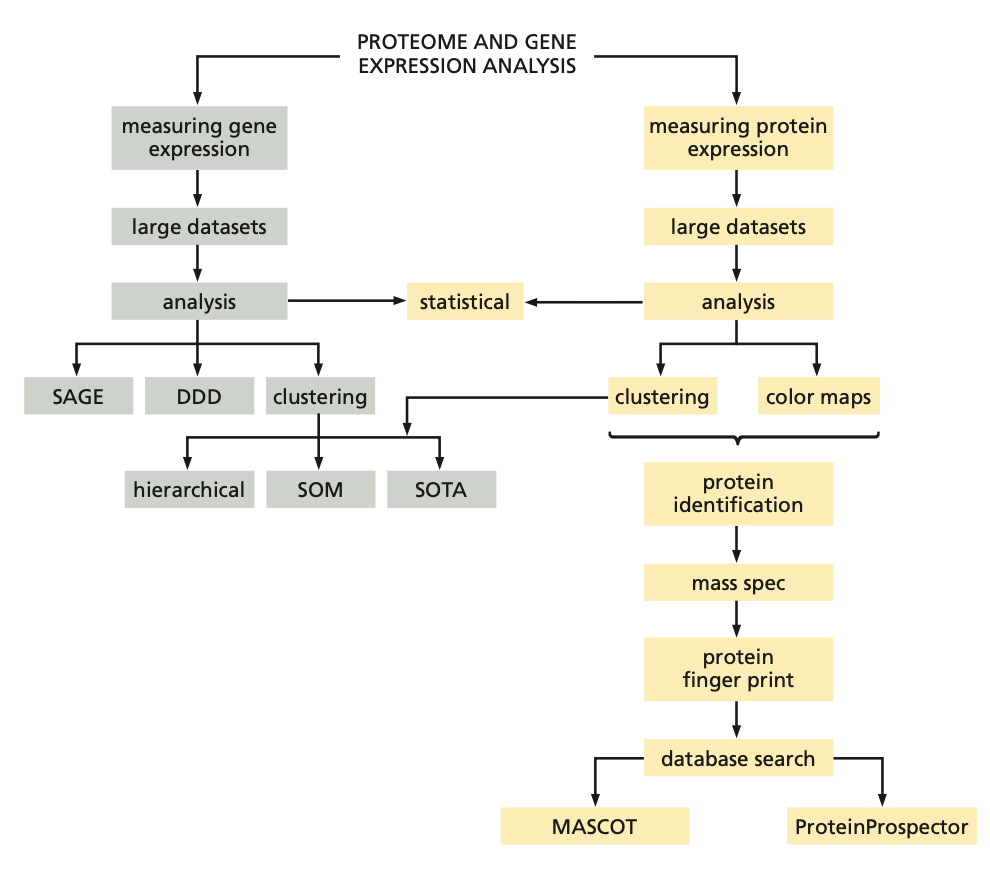
\includegraphics[width=0.5\textwidth]{Overlaping.png}
    \caption{\label{fig:Overlaping}Describing some experimental aspects of protein expression and of the analysis of the resulting data.~\cite{zvelebil_understanding_2008}.}
\end{figure}

For functional protein, mRNAs need to be translated, whilst the protein products can change which influence their function. For this reason we can measure and anlayse different proteins. 

There is more proteins than there are genes in a genome. Transcripts can be spliced in various ways to give different mRNAs, providing different protein products, from the same gene. However, proteins that can be modified after translation giving more different protien products.

Protien expressions can vary in a organism depending on the origin and it will also differ between the separate stages of an organism’s life cycle and under different environmental conditions. 

\begin{definition}[proteome]
    The proteome refers to all the proteins that make up an organism at a specific point in time and under specific conditions.
\end{definition}

It is important to know how protein expression is affected in order to understand how an organism or a cell functions~\cite{zvelebil_understanding_2008}.

\subsection{RNAseq}

The transcriptome is important for revealing the molecular constituents of cells and tissues, interpreting the functional aspects of the genome, also for understanding development and disease~\cite{wang_rna-seq_2009}.

Many methods deduce and quantify the transcriptome, including hybridization or sequence-based approaches. For example, hybridization-based approaches involve incubating fluorescently labeled cDNA with microarrays or commercial high-density oligo microarrays~\cite{wang_rna-seq_2009}.

However, these methods have several limitations, such as: 
\begin{itemize}
    \item Dreliance upon existing knowledge about genome sequence.
    \item Limited dynamic range of detection owing to both background.
    \item High background levels owing to cross-hybridization~\cite{okoniewski_hybridization_2006}~\cite{royce_toward_2007}.
    \item saturation of signals.
\end{itemize}

\begin{definition}[transcriptome]
    The transcriptome is the complete set of transcripts in a cell, and their quantity, for a specific developmental stage or physiological condition. 
\end{definition}

Sequence-based approaches directly determine the cDNA sequence such as Tag-based methods which include SAGE, CAGE~\cite{kodzius_cage_2006}, MPSS~\cite{reinartz_massively_2002}.

Each approach is high throughput and can provide precise, gene expression levels. However, a significant portion of the short tags can not be uniquely mapped to the reference genome~\cite{wang_rna-seq_2009}.

RNA-Seq RNA sequencing has clear advantages over existing approaches it uses deep sequencing technologies where a population of RNA is converted to a library of cDNA fragments with adaptors attached to one or both ends. Each molecule is then sequenced in a high-throughput manner to obtain short sequences from one or both ends~\cite{wang_rna-seq_2009}.

\begin{figure}[H]
    \centering
    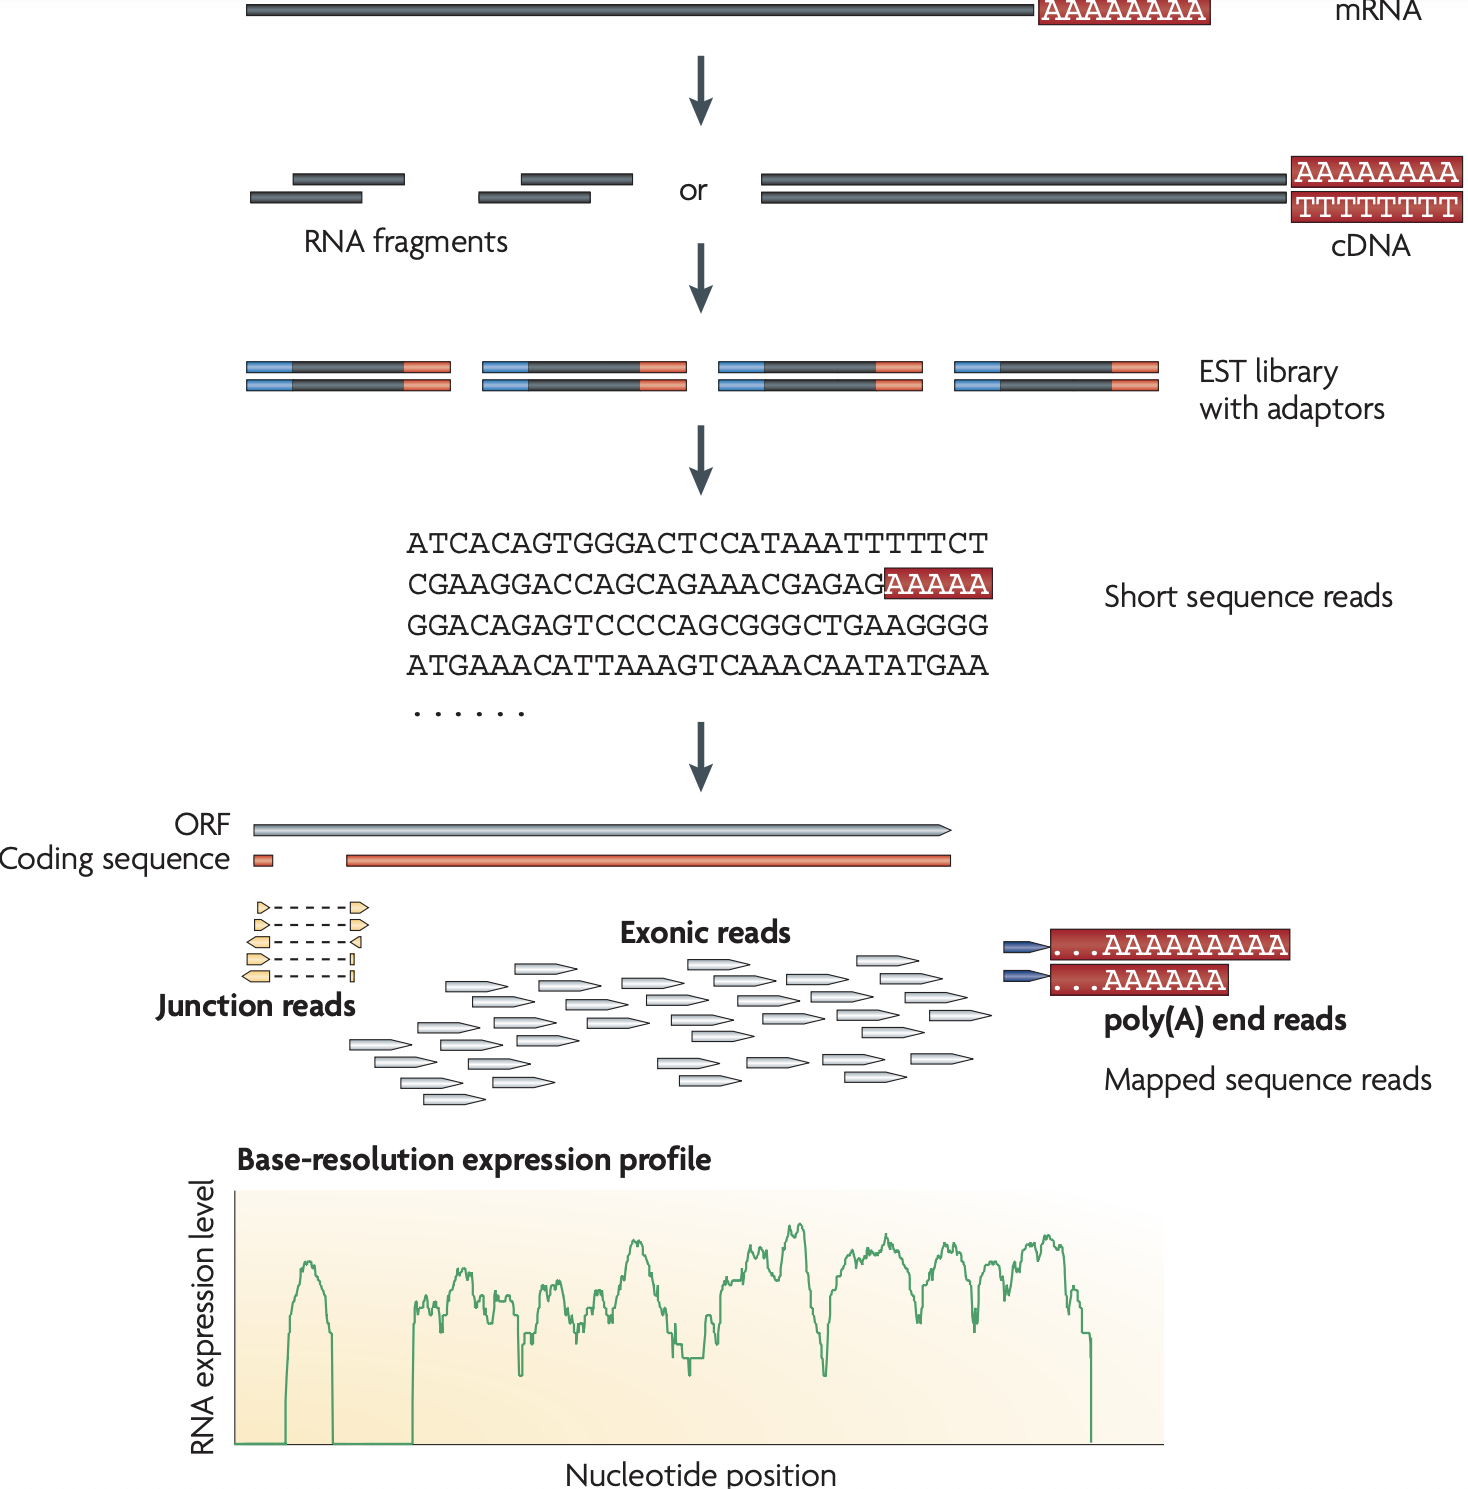
\includegraphics[width=0.5\textwidth]{RNAseq.png}
    \caption{\label{fig:RNAseq}A typical RnA-seq experiment. RNAs are first converted into a library of cDNA fragments through either RNA fragmentation or DNA fragmentation. Sequencing adaptors are subsequently added to each cDNA fragment and a short sequence is obtained from each cDNA using high-throughput sequencing technology. The resulting sequence reads are aligned with the reference genome or transcriptome.}
\end{figure}

\subsection{Alpha Fold}

AlphaFolds' goal is to predict the 3D coordinates of all heavy atoms for a given protein using the primary amino acid sequence and aligned sequences of homologues as inputs~\cite{jumper_highly_2021}.

Mutations in proteins can lead to misfolding which is often associated with disease states, for example, Alzheimer’s and Parkinson’s which is one of the challenges for alphaFold~\cite{felix_brief_nodate}.

The output is a file containing the 3D coordinates for every non-hydrogen atom in the protein. whilst showing the confidence levels for every amino acid residue, providing the reliability of the predicted structure~\cite{felix_brief_nodate}.

\subsubsection{Bioinformatics with Alpha Fold}

In July 2021, AlphaFold was developed by DeepMind and was made available to
the public~\cite{tunyasuvunakool_highly_2021}. 

Where it tries to solve the issue of invariant protein structures that are under translations and rotations~\cite{baldi_principled_nodate}.

AlphaFold is trained on protein chains from the PDB using the input sequence to query databases of protein sequences to generate a multiple sequence alignment~\cite{jumper_highly_2021}. Although we still do not exactly know how a protein sequence folds and alpha fold do not help in figuring this out its impact will likely be in accelerating and improving the production of new medications~\cite{nussinov_alphafold_2022}.


\subsubsection{AlphaFold 2}

The CASP14 was recently held which is a blind trial that critically assesses
techniques for protein structure prediction~\cite{david_alphafold_2022}, AlphaFold2 was entered and out-performed all competitors. 

Recently, RoseTTAFold was developed, trying to implement similar principles. Since then, other end-to-end structure predictors have emerged using different principles such as fast multiple sequence alignment processing in DMPFold218 and language model representations.\cite{bryant_improved_2022}.

We use the root mean square deviation, to calculate the similarity between the two structures, AlphaFold models had an accuracy of 0.96 compared to 2.80 which was the second-best score. AlphaFold models also had a high level of accuracy in predicting the position of residue side chains when the protein backbone prediction was accurate~\cite{david_alphafold_2022}~\cite{jumper_highly_2021}.


\section{The Protein Data Bank and the File Formats}

\subsection{Protein Data Bank}

The Protein Data Bank was established at Brookhaven National Laboratories ~\cite{bernstein_protein_1977} in 1971 as an archive for biological macromolecular crystal structures~\cite{berman_protein_2000}.

\begin{definition}[Macromolecular]
    Macromolecular is any very large molecule, usually with a diameter ranging from about 100 to 10,000 angstroms
\end{definition}

It is an information source for data retrieved from atomic structures, crystallography, and three-dimensional structures of biomolecules, including nucleic acids and proteins~\cite{behzadi_worldwide_2021}. 

At the time this was the first open-access digital data resource in biology which started with just seven protein structures~\cite{burley_rcsb_2022}.

Various groups such as the Protein Data Bank in Europe, Protein Data Bank Japan help manage the Protein Data Bank archive. Current wwPDB members also include the ElectronMicroscopy Data Bank and the Biological Magnetic Resonance Bank~\cite{burley_rcsb_2022}.

Protein Data Bank China has recently joined the wwPDB as an Associate Member with its role as wwPDBdesignated PDB Archive Keeper. Where they are responsible for weekly updates of the archive and safeguarding both digital information and a physical archive of correspondence~\cite{burley1_rcsb_2022}.

The management of PDB must comply with FAIR (the acronym depicts: Findable, Accessible, Interoperable, Reusable) and FACT~\cite{van_der_aalst_responsible_2017} guiding principles for scientific data~\cite{wilkinson_fair_2016}~\cite{westbrook_impact_2020}.

\begin{table}[h!]
    \begin{center}
    \label{tab:FAIR}
        \begin{tabular}{c|p{0.65\linewidth}}
        The FAIR Guiding Principles\\
        \hline
        \\
        To be Findable: & F1. (meta)data are assigned a globally unique and persistent identifier\\
        & F2. data are described with rich metadata (defined by R1 below)\\ & F3. metadata clearly and explicitly include the identifier of the data it describes\\ & F4. (meta)data are registered or indexed in a searchable resource\\
        \\
        \hline
        \\
        To be Accessible: & A1. (meta)data are retrievable by their identifier using a standardized communications protoco\\
        & A1.1 the protocol is open, free, and universally implementable\\ & A1.2 the protocol allows for an authentication and authorization procedure, where necessary\\ & A2. metadata are accessible, even when the data are no longer available
        \\
        \hline
        \\
        To be Interoperable: & I1. (meta)data use a formal, accessible, shared, and broadly applicable language for knowledge representation.\\
        & I2. (meta)data use vocabularies that follow FAIR principles\\ & I3. (meta)data include qualified references to other (meta)data\\
        \\
        \hline
        \\
        To be Reusable: & R1. meta(data) are richly described with a plurality of accurate and relevant attributes\\
        & R1.1. (meta)data are released with a clear and accessible data usage license\\ & R1.2. (meta)data are associated with detailed provenance\\ &
        R1.3. (meta)data meet domain-relevant community standards\\
        \end{tabular}
        \caption{\label{Fair}The guidlines to what builds up the FAIR principles~\cite{wilkinson_fair_2016}}
    \end{center}
\end{table}

\subsubsection{Aims and Objectives of PDB}

Enzymology, electron microscopy, computational chemistry small molecule crystallography, biochemistry, biophysics, macromolecular crystallography and nuclear magnetic resonance spectrometry all help the aims and goals of the PDB archive~\cite{behzadi_worldwide_2021}.

\begin{definition}[Enzymology]
    Enzymology is the branch of biochemistry aiming to understand how enzymes work
\end{definition}

\begin{definition}[Electron Microscopy]
    Electron microscopy is a technique for obtaining high resolution images of biological and non-biological specimens.
\end{definition}

PDBs provide open access to nearly 200 000 archived, validated, and biocurated experimentally determined three-dimensional structures of biological macromolecules.3D structures archived in the PDB have enabled important scientific breakthroughs by basic and applied researchers~\cite{burley_impact_2021}. Open access to PDB data without restrictions on usage has also aided structural bioinformatics in areas such as computational biology.

\subsubsection{Timeline of PDB}

I have provided a timeline representing the milesstones achived within the protein data bank. Where PDB marked its 52st anniversary of continuous operations.

\begin{chronology}{1971}{1981}{90ex}
    \event{1971}{PDB established}
    \event{1973}{Early structures include}
    \event{1974}{First tRNA structures}
    \event{1979}{First Z-DNA published}
    \event{1981}{First B-DNA in the PDB}
\end{chronology}

\begin{chronology}{1989}{2001}{90ex}
    \event{1989}{IUCr policy and First NMR structure}
    \event{1991}{First 3DEM structure}
    \event{\decimaldate{1}{11}{1994}}{First PDB Web Browser}
    \event{\decimaldate{1}{5}{1996}}{25th Anniversary and Release of AutoDep}
    \event{\decimaldate{1}{10}{1998}}{10,000th structure is released}
    \event{2000}{Osaka center and First ribosome structures}
    \event{\decimaldate{1}{7}{2001}}{EMDB established at MSD-EBI}
\end{chronology}

\begin{chronology}{2003}{2011}{90ex}
    \event{2003}{wwPDB established by RCSB, PDBe, PDBj}
    \event{\decimaldate{1}{10}{2004}}{Last postal PDB archive}
    \event{2006}{BMRB joins wwPDB}
    \event{\decimaldate{1}{11}{2006}}{First release of remediated data}
    \event{\decimaldate{1}{7}{2008}}{50,000th structure and Deposition of (X-ray, NMR)}
    \event{\decimaldate{1}{10}{2009}}{Deposition chemical shift and Worldwide PDB Foundation established}
    \event{2011}{PDB40 Symposium and First structure X-ray Free Electron Laser}
\end{chronology}

\begin{chronology}{2012}{2021}{90ex}
    \event{\decimaldate{1}{5}{2012}}{Validation Reports}
    \event{\decimaldate{1}{4}{2013}}{Large structures PDBx/mmCIF}
    \event{2014}{OneDep and 100,000+ structures}
    \event{\decimaldate{1}{3}{2015}}{Reports NMR, 3DEM and Deposition of EM maps}
    \event{\decimaldate{1}{4}{2016}}{PDB-Dev and PDB Entry Versioning}
    \event{\decimaldate{1}{2}{2017}}{ligand validation and 150,000+ structures}
    \event{\decimaldate{1}{11}{2018}}{First SARS-CoV-2 structure }
    \event{\decimaldate{1}{6}{2019}}{Reports for 3DEM coord, maps}
    \event{\decimaldate{1}{12}{2019}}{Alphafold2 and carbohydrate data}
    \event{2021}{PDB50 and EMDB partner in wwPDB}
\end{chronology}

\subsubsection{Recent Project}

A project was undertaken to change the information management services for RCSB.org. The idea was to have developed a primary place for studying 3D biostructures by extending RCSB.org web portal functionality to support parallel delivery of more than one million CSMs publicly available from AlphaFold DB and ModelArchive together~\cite{burley1_rcsb_2022}.

\subsubsection{Covid}

During the COVID-19 pandemic, more than 2000 structures associated with the agent of the coronavirus disease were released and have become accessible to global users for free. The properties of these structures give us this opportunity to find out the ligand binding sites, the spatial conformation of ligands, protein-to-protein interactions, and amino acid substitutions regarding different viral proteins. Moreover, chemical, functional and energetic characteristics can also be gained to describe the potential capabilities of each molecule. These properties might aid us to determine the potential drug targets for drug design and vaccine preparation~\cite{lubin_evolution_2020}.

\subsection{PDB Currently}

As of 2022, the PDB has a vast number of 3D biostructures, eukaryotic protein structures exceeded 105 000. Bacterial protein structures were also numerous, totaling nearly 66 000. Archaeal protein structures were the least numerous totaling 5500. However the PDB coverage is decidedly limited, with mouse protein structures being most numerous at 8000 structures~\cite{burley_open-access_2021}. 

We have powerful tools developed by RCSB PDB for searching and analysis which include structure, sequence, sequence motif, structure motif, and visualization~\cite{burley1_rcsb_2022}.

Upon reaching the RCSB.org home page, users can query, organize, visualize, analyse, compare, and explore PDB structures and CSMs side-by-side. Searching 3D structure information can encompass PDB structures and CSMs or be limited to PDB structures only. Either PDB structures or CSMs can be excluded from the search results. The two types of structure information accessible via RCSB.org are clearly distinguished from each other. Top bar searching and data delivery for PDB structures and CSMs~\cite{burley1_rcsb_2022}.

\subsubsection{The PDB Site currently}

\begin{figure}[H]
    \centering
    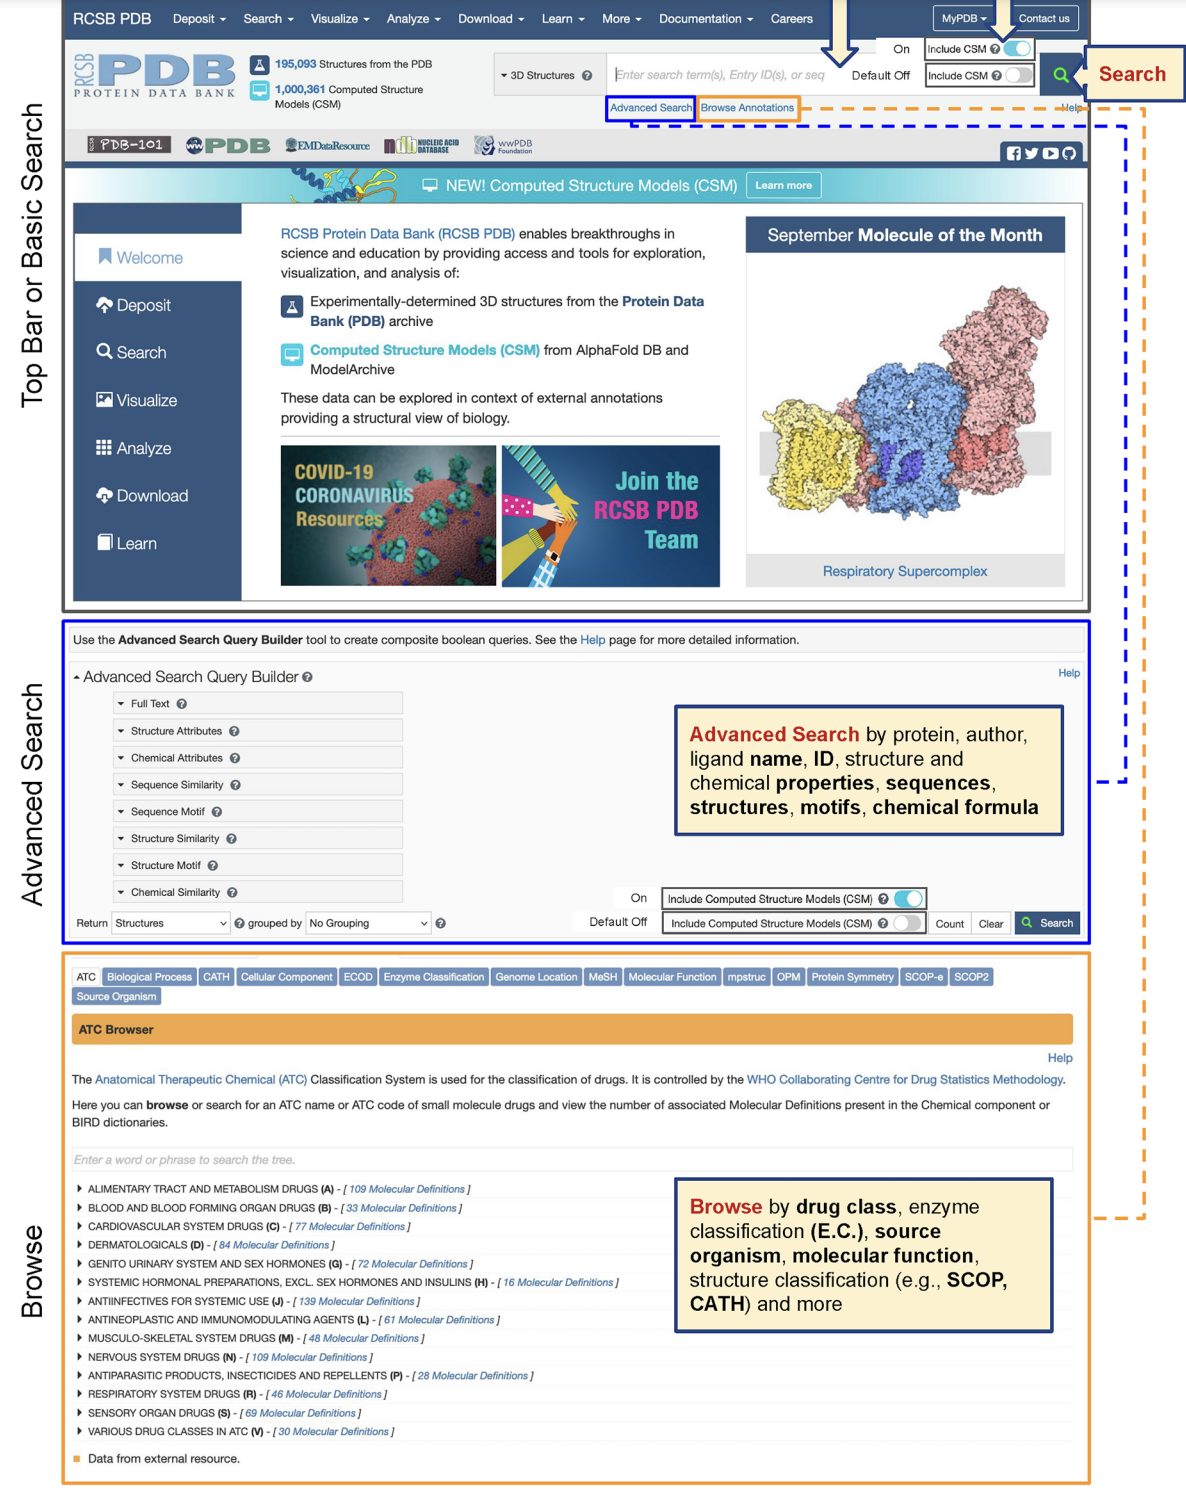
\includegraphics[width=0.5\textwidth]{PDB Site.png}
    \caption{\label{fig:PDB}Search options at RCSB.org include Top Bar or Basic Search; Advanced Search; and Browse Annotations~\cite{burley1_rcsb_2022}.}
\end{figure}

\begin{figure}[!h]
    \centering
    \begin{subfigure}[t]{.45\textwidth}
        \centering
        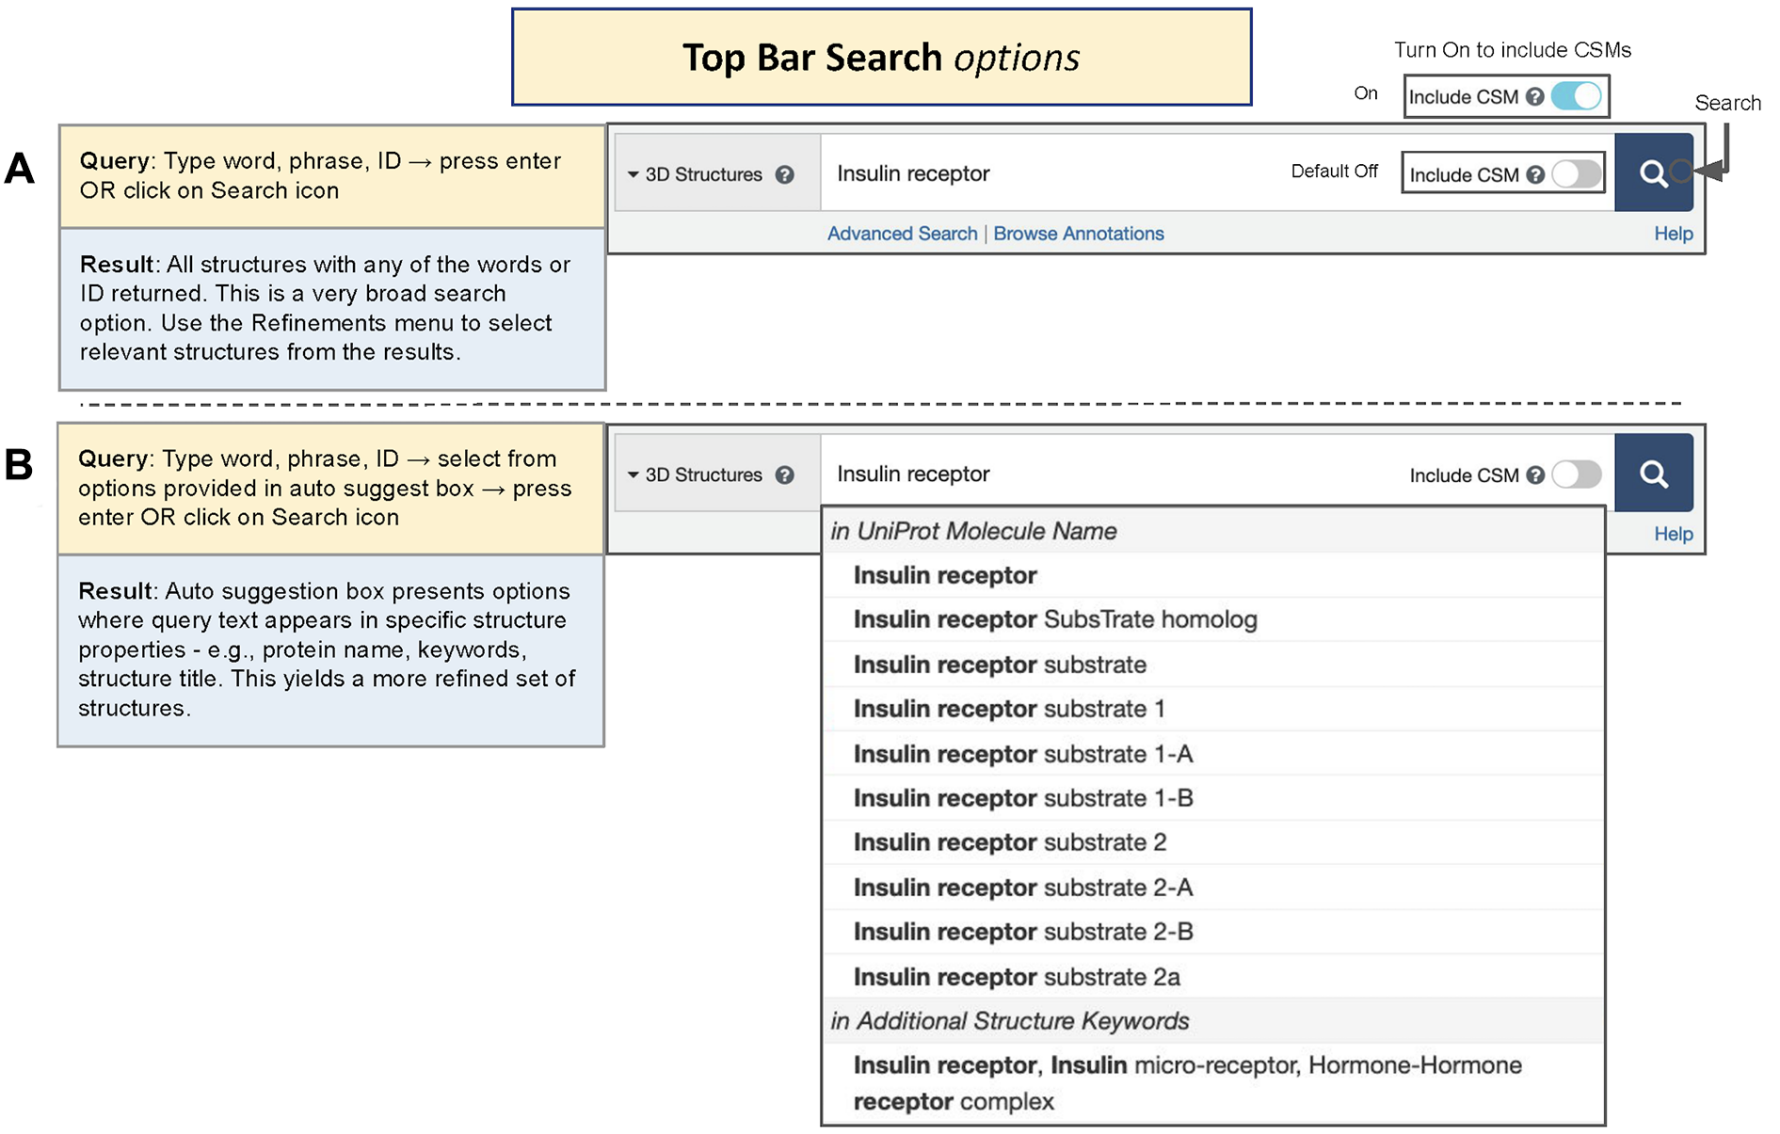
\includegraphics[width=0.9\textwidth]{Top Bar Search A.png}
        \caption{}
        \label{fig:Top1} 
    \end{subfigure}
    \begin{subfigure}[t]{.45\textwidth}
       \centering
       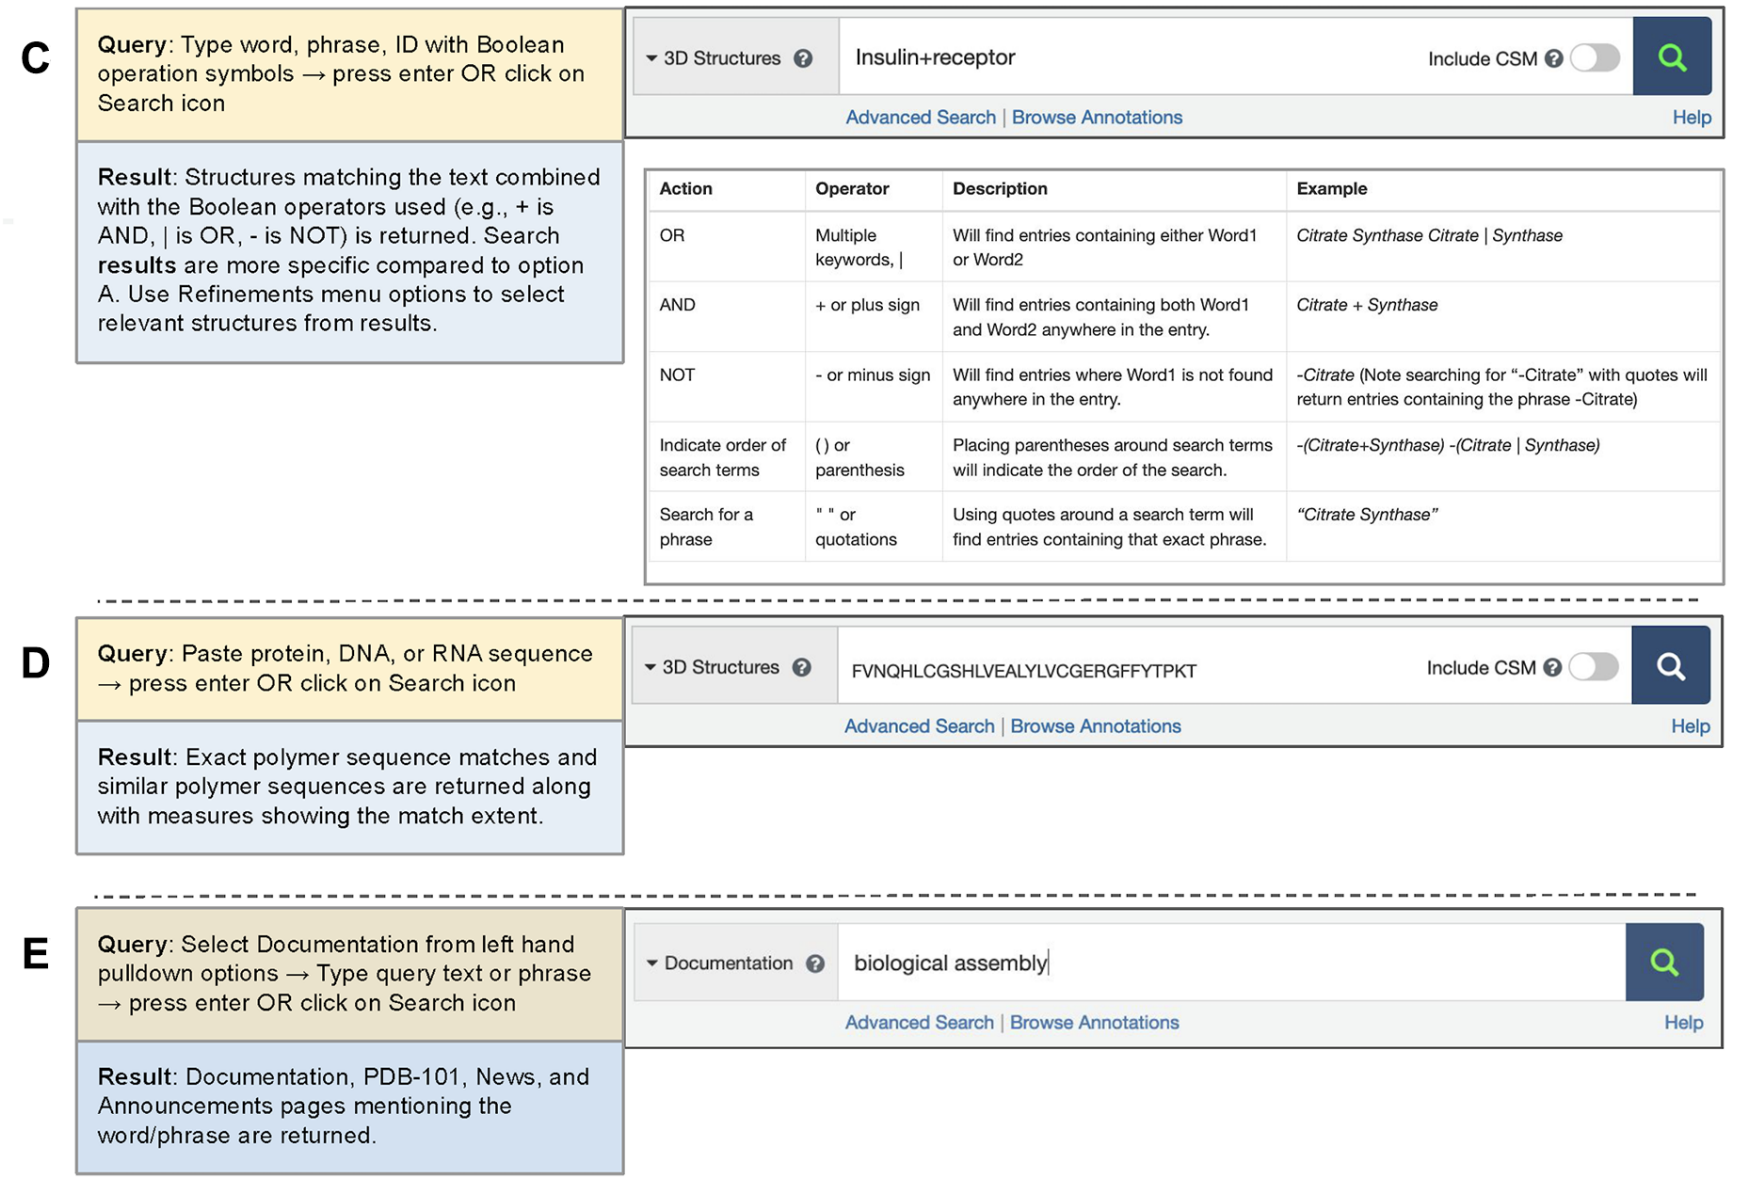
\includegraphics[width=0.9\textwidth]{Top Bar Search B.png}
       \caption{}
       \label{fig:Top2}
    \end{subfigure}
    \caption{\emph{Top Bar or Basic Search options available from every RCSB.org web page. Examples of searching for 3D structures using (A) simple text string insulin receptor; (B) drop down autosuggestions based on the text string insulin receptor; (C) Boolean operators to combine insulin + receptor (+ = AND); or (D) an amino acid sequence. (E) Searching RCSB.org documentation using a text string biological assembly~\cite{burley1_rcsb_2022}}}
    \label{fig:SAGE}
\end{figure}

\subsection{Recent Improvements}

\subsubsection*{Recent RCSB PDB data architecture improvements}

In 2020, RCSB PDB had an upgrade of its delivery architecture~\cite{rose_rcsb_2021}at RCSB.org~\cite{powerful_rcsb_2021}. The legacy monolithic data delivery application was changed into a distributed deployment of individual microservices, each with a single responsibility. Data access services provide both Representational State Transfer and GraphQL API access to a data warehouse hosted in a MongoDB documentoriented database. Originally, advanced Search QueryBuilder functionality encompassed text, PDB data attributes, 3D structure, sequence, biopolymer sequence motif, and chemical similarity. Every search function is implemented as an independent service. A separate search service is responsible for launching each search function, combining and delivering their integrated results to public programmatic search APIs. When each service has a single responsibility, we have greater flexibility in scaling the deployment of services in response to changes in user load and significant reductions in the time required to develop, test, and deploy new features. The Sequence Motif search function has been extended with a new 3D Structure Motifsearch capability~\cite{bittrich_real-time_2020}. 

\subsubsection*{Recent advances in RCSB PDB data integration}

RCSB PDB integrates the content of each expertly biocurated Entry with information from more than 50 external data resources. 

Integrated external data needs to follow a data schema that defines the organization of the RCSB PDB data warehouse. Finally, it is available to RCSB PDB front-end services, public data access APIs, and our text search indexing service~\cite{burley_rcsb_2022}.

\begin{table}[h!]
    \begin{center}
    \label{tab:External Data}
        \begin{tabular}{c|p{0.58\linewidth}}
        External Resources\\
        \hline
        \\
        AlphaFold DB & Computed Structure Models by AlphaFold2
        \\
        \hline
        \\
        ATC & 	Anatomical Therapeutic Chemical (ATC) Classification System from World Health Organization
        \\
        \hline
        \\
        Binding MOAD & Binding affinities
        \\
        \hline
        \\
        Binding DB & Binding affinities
        \\
        \hline
        \\
        BMRB & BMRB-to-PDB mappings
        \\
        \hline
        \\
        Cambridge structural Database & Crystallographic small molecule data from the Cambridge Crystallographic Data Centre
        \\
        \hline
        \\
        CATH & 	Protein structure classification- Class, Architecture, Topology/fold, and Homologous superfamily    
        \\
        \hline
        \\
        ChEMBL & Manually curated database of bioactive molecules with drug-like properties
        \\
        \hline
        \\
        CSD & Cambridge Structural Database: Validated and curated small-molecule organic and metal-organic crystal structures from the Cambridge Crystallographic Data Centre
        \\
        \hline
        \\
        DrugBank & Drug and drug target data
        \\
        \hline
        \\
        ECOD & Evolutionary Classification of Protein Domains
        \\
        \hline
        \\
        EMDB & 3DEM density maps and associated metadata
        \\
        \hline
        \\
        ExplorEnz & IUBMB Enzyme nomenclature and classification
        \\
        \hline
        \\
        Gencode & Human and Mouse Gene annotations
        \end{tabular}
        \caption{\label{External Data}Some of the External Resources Integrated Into RCSB PDB}
    \end{center}
\end{table}



\subsubsection*{Recent PDBx/mmCIF data standard improvements}

The PDBx/mmCIF data standard is maintained by the wwPDB organization in collaboration with wwPDBPDBx/mmCIF Working Group domain experts recruited from the scientific community. The PDBx/mmCIF web resource supports browse and search access to standard terminology. The Working Group includes developers for many of the widely used structure determination software systems, who ensure that data produced by these programs comply with the PDBx/mmCIF data standard, generating complete and correct data files for PDB deposition. The wwPDB and the Working Group collaborate on developing terminologies for new and rapidly evolving methodologies such as Free Electron Laser, 3DEM, Serial Crystallography, and X-ray, whilst improving representations for existing data content. Most recently, the Working Group has focused on modernizing content descriptions for processed X-ray diffraction data, including extensions describing anisotropic diffraction limits, unmerged reflection data, and new quality metrics of anomalous diffraction data. Deposition and delivery improve our ability to assess experimental data quality, and every PDB data consumer's ability to Find and Reuse relevant PDB Entries~\cite{burley_rcsb_2022}.

\subsection{Summary}
\subsubsection{Future and struggles of PDB}
\subsubsection{Future}
As the PDB archive has started its 52nd year, it gives open access to analyses of structures and much more to: basic and applied researchers, educators, and students spanning fundamental biology, biomedicine, bioenergy, bioengineering, and biotechnology, with key points that help many communities that use this facility. Firstly It delivers Data In and Data Out services efficiently to a user base that is now numbering many millions worldwide. Secondly, it has wwPDB partners that process, validate, and biocurate the growing number of increasingly complex PDB depositions received. Manages and safeguards the growing PDB archive in its role as wwPDB designated Archive Keeper. Thirdly it enables searching, visualization, exploration, and analysis of experimentally-determined PDB structures integrated with more than one million CSMs through its web portal.~\cite{burley1_rcsb_2022}.

\subsubsection{Struggles}
Even after all the advancments PDB has gone through there are still additional challenges lying ahead which include:

\begin{itemize}
    \item Rapid growth in public-domain CSMs of individual polypeptide chains, already numbering >200 million at the time of writing.
    \item Anticipated advances in AI/ML-based prediction of structures of multi-protein complexes.
    \item Continued development of biomolecular structure determination methods using X-ray Free Electron Lasers, revealing the microscopic details of chemical reactions in real time.
    \item Growth in the number and complexity of atomic-level cryoelectrontomography structures of macromolecular machines.
    \item Integration of PDB structures and CSMs with complementary information coming from correlative light microscopy and related imaging methods across length scales ranging from atoms to small molecules to individual biomolecules to macromolecular assemblies to organelles to cells and ultimately tissues
    \item Merging of the PDB-Dev prototype archiving system for integrative methods structures with the PDB archive
    \item Federating other biodata resources, such as the SmallAngle Scattering Database and the Proteomics Identification Database, with the PDB, EMDB and BMRB core archives jointly managed by the wwPDB partnership
\end{itemize}
~\cite{burley1_rcsb_2022}.

\subsection{File Formats}

The PDB archive holds a few different types of file types that hold data such as atomic coordinates and other information describing proteins and other biological macromolecules. Depending on what the data is created from it can fall into a different category.

\subsubsection{PDB Data}

The main information in the PDB archive is coordinate files for biological molecules. These files list the atoms in each protein and their 3D coordinates.

These files are available in several formats:

\begin{itemize}
    \item PDB
    \item mmCIF
    \item XML
\end{itemize}

The header section of the text summarizes the protein, citation information, and the details of the structure solution, which is then followed by the sequence and a long list of the atoms and their coordinates. It also contains the experimental observations used to determine atomic coordinates~\cite{noauthor_pdb101_nodate}.

\subsubsection{.pdb Files}

The PB format consists of a collection of records that describe the atomic coordinates, chemical and biochemical features, and experimental details of the structure determination~\cite{westbrook_pdb_2003}.

Each item of data in the PDB format is assigned to a one of PDB record types (HEADER. SOURCE. REMARK, etc.). The ATOM records the atomic coordinate data~\cite{westbrook_pdb_2003}.

PDB format has been extended with new REMARK records. For example, REMARK 3 that encodes refinement information has been modified and extended for each new refinement program and program version~\cite{westbrook_pdb_2003}.

The PB format uses fixed-width fields to represent data, so we have limits on the size of certain items of data. For example, we cant have more then 99,999 atoms and polymer chain can be only one character. This means some structures are devided into multiple files~\cite{westbrook_pdb_2003}.

\begin{figure}[H]
    \centering
    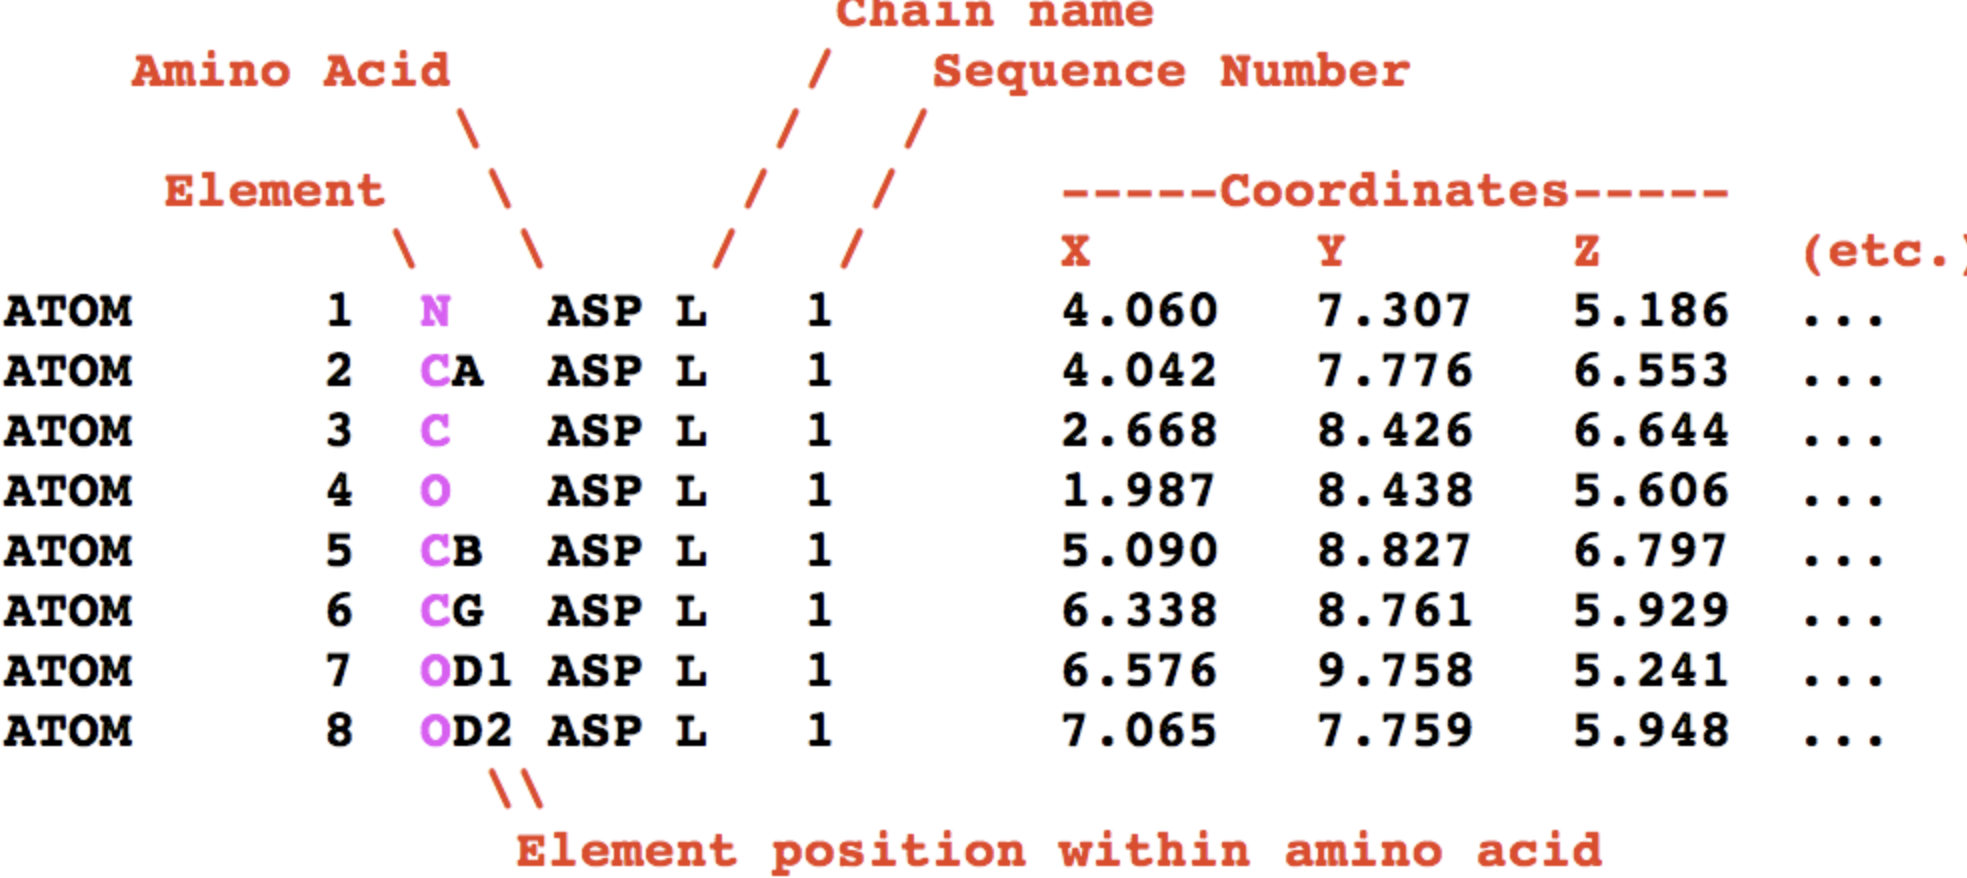
\includegraphics[width=0.5\textwidth]{PDB File.png}
    \caption{\label{fig:PDB file}Showing contents of a PDB file for the Atom values~\cite{adams_announcing_2019}.}
\end{figure}

\subsubsection{.mmCIF Files}
Mmcif is a dictionary-based approach to data extracted from crystallographic experiments~\cite{westbrook_pdb_2003}.

It includes all the data we can find in a pdb file. Also, we have sufficient data names so that the experimental section of a structure paper can be written automatically and to facilitate the development of tools i.e. computer programs could easily access and validate mmCIF data files~\cite{westbrook_pdb_2003}.

\subsubsection{.xml}

XML builds from a PDB Exchange dictionary. Although presented in very different syntaxes, the PDB Exchange and XML representations use the same logical data organization.~\cite{westbrook_pdbml_2005}.

The dictionary data block is mapped to the standard top-level XML schema element, and the data file data block is mapped to a datablock element. Category or table definitions in the Exchange dictionary are described as XML complex types. The category definition.~\cite{westbrook_pdbml_2005}.

\begin{figure}[H]
    \centering
    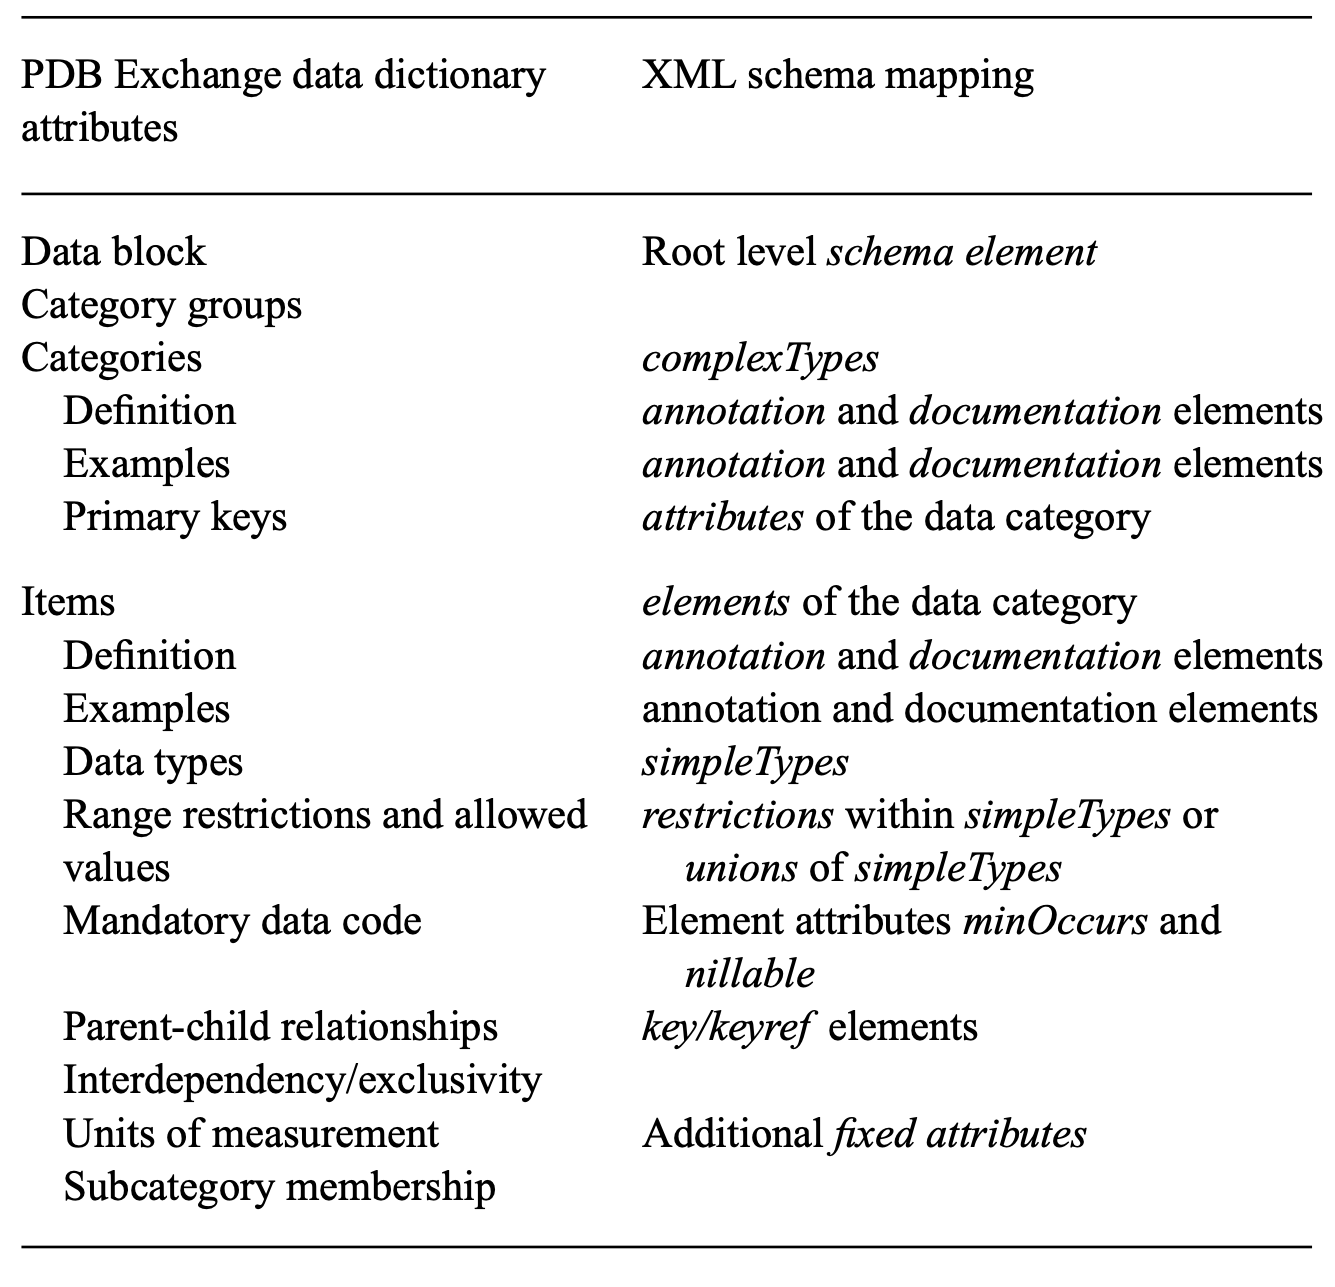
\includegraphics[width=0.5\textwidth]{xml.png}
    \caption{\label{fig:xml}Summary of the correspondences between PDB Exchange data dictionary and XML schema metadata~\cite{westbrook_pdbml_2005}.}
\end{figure}


\subsubsection{Visualizing Structures}

PDB files can be viewed from text editors but we can also use a browsing or visualization program. RCSB PDB allows you to search and explore the information, including information on experimental methods and the chemistry and biology of the protein. Visualization programs allow to read of the PDB file and, display the protein structure generating custom pictures of it. These programs can contain analysis tools that allow you to measure distances and bond angles, and identify interesting structural features~\cite{noauthor_pdb101_nodate}.
\subsubsection{Reading Coordinate Files}

Before exploring structures in the PDB archive we need some prior understanding of the coordinate files. For example, we can find a diverse mixture of biological molecules, small molecules, ions, and water which can get confusing we can use the names and chain IDs to help sort these out. In structures determined from crystallography, atoms are annotated with temperature factors that describe their vibration and occupancies that show if they are seen in several conformations. NMR structures often include several different models of the molecule~\cite{noauthor_pdb101_nodate}.

\subsubsection{Potential Challanges}

There are some things to note as you could fall into some challenges when browsing through the PDB archive. Many structures, particularly those determined by crystallography, only include information about part of the functional biological assembly. One thing to note is that the PDB can aid with this. Another note is many PDB entries are missing portions of the molecule that were not observed in the experiment. These include structures that include only alpha carbon positions, structures with missing loops, structures of individual domains, or subunits from a larger molecule. In addition, most of the crystallographic structure entries do not have information on hydrogen atoms~\cite{noauthor_pdb101_nodate}.


\section{Hadoop spark and pyspark}

\subsubsection{What is Hadoop}

Hadoop is an open-source framework for writing and running distributed applications that process large amounts of data.  Key aspects making it valuable such 1. Accessible 2.Robust 3. Scalable 4.simple~\cite{lam_hadoop_2010}.

HDFS is used in haddop which is a filessystem and a MapReduce engine. With one master node and many worker nodes. The master node provides instructions to the worker nodes and computations are performed on the worker nodes.~\cite{hazarika_performance_2017}.

\subsubsection{Mapper}
Input key/value pairs are mapped to a set of key/value pairs. The mapper then sorts the key-value pairs by the keys. Partitioners are mainly responsible for providing intermediate key/values to the reducers~\cite{patel_addressing_2012}~\cite{hazarika_performance_2017}.

\subsubsection{Reducer}

Firstly, the reducer combines data having the same key from different map functions. The values having the same key are reduced to a smaller set of values and output is produced~\cite{hazarika_performance_2017}.

\subsubsection{What is Spark}
Apache Spark is a popular open-source platform for large-scale data processing used for iterative machine learning tasks~\cite{meng_mllib_2016}.

Spark is a cluster computing system providing APIs in Java, Scala, Python (pySpark), and R, along with an optimized engine that supports general execution graphs. Moreover, Spark is efficient at iterative computations so it is suited for the development of large-scale machine learning applications~\cite{meng_mllib_2016}.

Spark is a quick and general engine used for analysing large-scale data stored across a cluster of computers. Spark uses in-memory cluster computing which is its most important feature for increasing the processing speed of an application. It combines SQL streaming and complex analytics~\cite{hazarika_performance_2017}.

\subsubsection{Spark vs Hadoop}

\begin{table}[h!]
    \begin{center}
    \label{tab:Amino acids}
        \begin{tabular}{p{0.6\linewidth}|p{0.35\linewidth}}
        Hadoop Map Reduce & Spark\\
        \hline
        \\
        For Applications that repeatedly reuse the same set of data, map reduce is very inefficient. & Spark uses in-memory processing, reusing it for faster computation.
        \\
        \hline
        \\
        MapReduce is quite faster in batch processing. & As memory size is limited, it would be quite slower in batch processing of huge data set.
        \\
        \hline
        \\
        Data is stored in disk for processing. & Data is stored in main memory. As it is an inmemory computation engine entire data is copied. 
        \\
        \hline
        \\
        Difficulty in processing and modifying data in real time due to its high latency. & Used to process and modify data in real time due to its low latency. 
        \\
        \hline
        \\
        Predominantly used to process from bygone datasets. & Predominantly used for streaming, batch processing and machine learning
        \\
        \hline
        \\
        For fault tolerance, MapReduce uses replication. & For fault tolerance, Spark uses RDDs.
        \\
        \hline
        \\
        It merges and partitions shuffle files. & It does not merges and partition shuffle files. 
        \\
        \hline
        \\
        Primarily disk based computation. & Primarily RAM based computation.
        \\
        \end{tabular}
        \caption{\label{hadoopvsspark}Showing the differences between haddop and spark~\cite{hazarika_performance_2017}.}
    \end{center}
\end{table}

\begin{table}[h!]
    \begin{center}
    \label{tab:Amino acids}
        \begin{tabular}{c|cc}
        Number of words & Hadoop (Sec) & Spark(Sec)\\
        \hline
        \\
        100 & 79 & 28.841
        \\
        1000 & 91 & 31.185
        \\
        10000 & 96 & 35.181
        \\
        100000 & 103 & 36.969
        \\
        1000000 & 116 & 39.569
        \end{tabular}
        \caption{\label{Results1}Comparision of Execution time for wordcount program~\cite{hazarika_performance_2017}.}
    \end{center}
\end{table}

\begin{table}[h!]
    \begin{center}
    \label{tab:Amino acids}
        \begin{tabular}{c|cc}
        Number of words & Hadoop (Sec) & Spark(Sec)\\
        \hline
        \\
        5 & 2.541 & 0.9030
        \\
        10 & 3.370 & 1.459
        \\
        50 & 6.420 & 2.840
        \\
        100 & 9.383 & 3.452
        \\
        200 & 10.100 & 5.749 
        \end{tabular}
        \caption{\label{Results1}Comparison of Execution time for logistic
        regression program~\cite{hazarika_performance_2017}.}
    \end{center}
\end{table}

Summarising the results shows Spark to be quicker in both experiments. Spark also provides an API for python which will be very helpful in this project seeing its easy nature to be able to read files and work with text-based files. Therefore I have decided to work with Pyspark for this project.

\subsubsection{Software Architectural Bottlenecks}

HDFS has scheduling delays in the architecture which results in cluster nodes waiting for new tasks as the access pattern is periodic.HDFS client code, serializes computation and I/O instead of decoupling and pipelining those operations.~\cite{shafer_hadoop_2010}.

\begin{definition}[HDFS]
    The Hadoop Distributed File System (HDFS) is a distributed file system designed to run on commodity hardware
\end{definition}

\subsubsection{Portability Limitations}
Some performance-enhancing features in the filesystem are not available such as bypassing the filesystem page cache and transferring data directly from the disk into user buffers. Thus, HDFS implementation runs less efficiently and has higher processor usage than would otherwise be necessary~\cite{shafer_hadoop_2010}.


\section{Software Development}

\subsection{Unit Tests}

I used unittest — Unit testing framework python API to help me test my code. The point of unit testing is to isolate each section of the program and show that the individual section is functioning correctly. The way I based my unit test was around each function I have in my PoC program. I then thought of several cases that could happen and ensured that I wrote a test for them. For example, I created a test to test a method that retrieves the PDB files in a folder. more specifically this test checked various things for example it checked to see that it contained all the files with the extension .pdb from the correct folder. To test this I added a different extension file into that folder and ran the test looking at the length of the output to see if it is correct. 

\begin{lstlisting}
    class TestGetAllPDBFiles(unittest.TestCase):
    directory = ("/Users/vinaykakkar/Desktop/PROJECT-main/
    ProofofConcepts/PDBontoaCluster/OriginalPDBs")

    def test_checktypeofpdbs(self):
        test = Lines.getallpdbfiles(self.directory)
        lis = []
        self.assertTrue(type(test) is type(lis))
    
    def test_checktypeofpdb(self):
        test = Lines.getallpdbfiles(self.directory)
        string = "string"
        self.assertTrue(type(test[0]) is type(string))

    def test_checknumberofpdbs(self):
        test = Lines.getallpdbfiles(self.directory)
        self.assertEqual(len(test), 2)

    def test_checkwrongdirectory(self):
        directory = ("Wrong")
        with self.assertRaises(Exception) as context:
            Lines.getallpdbfiles(directory)

\end{lstlisting}

Using these tests I made improvements to my code. For example, in the last test in the class TestGetAllPDBFiles, I check to see what happens if the directory provided is incorrect. At first, it errored with an ambiguous message which is not helpful. Once I ran the test I realized that I need to create a check to see if the directory exists and if it doesn't then throw a readable and understandable exception. Yeilding in my program is more robust.

\begin{lstlisting}
    def getallpdbfiles(directory):
    pdbfiles = []
    ## This line is checking to see if it exists first 
    ## before trying to get all the .pdb files
    if (Path(directory).is_dir()):
        for file in os.listdir(directory):
            filename = os.fsdecode(file)
            if filename.endswith(".pdb"):
                pdbfiles.append(filename)
    else:
        raise Exception("No files found: check Directory")
    return pdbfiles

\end{lstlisting}


\subsection{Branching}

The key role of branching is to allow more structure into the project which allows me to work on different aspects of a project at different times. As this project involves multiple parts for example when completing my tutorials on MapReduce I was already working on making a cluster for the first part of my PoC program. This gave me the freedom to easily work on different parts of the project very quickly. which allowed for a more structural progression compared to a linear block project progression such as completing the tutorial then completing the PoC the completing the reports in order.

\begin{figure}[H]
    \centering
    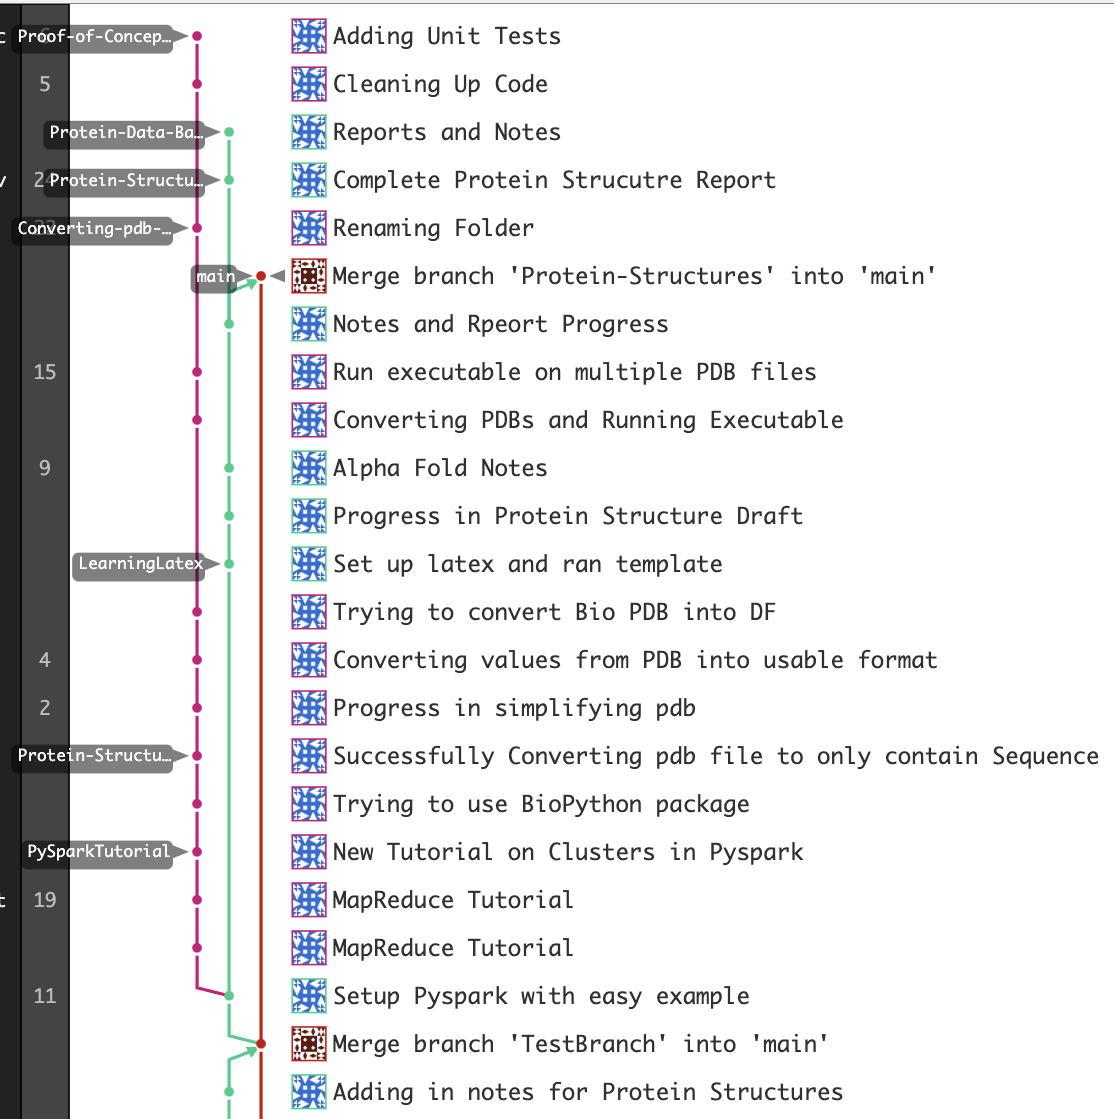
\includegraphics[width=0.5\textwidth]{Branching.png}
    \caption{\label{fig:Branching}Showing some branching of my gitlab project.}
\end{figure}

The main two splits I have when working on my project a for the Poc and Reports/Research. Branching will help even more in the second term as there will be more features to add to the program

\section{Planning and Time-Scale}

My planning and Time-Scale will be based on the objectives I have yet to complete and any extensions I decided to include in my project.

\subsection{Planning}

The second term will be mostly working on the program with not much more to research on the biology aspects of the project. I will get a new diary that will contain my thoughts and ideas also noting down the struggles face. Summarising the objectives to complete and extensions:

\begin{itemize}
    \item Provide some form of UI
    \item Perform/use user executables that are perfomred on pdb files which will yeild a result.
    \item Distribute clusters to multiple computers.
    \item Benchmarking.
    \item Mirror dataset from pdb site.
    \item Provide Guidelines for the executables.
    \item Improve UI
    \item A set of user executables that are ready and just need to be selected by the user.
    \item Implementation on a Public Mapreduce cluster e.g. Amazon.
\end{itemize}

I will also need to account for the final report and demo day presentation/poster at the end of the term.

\subsubsection{looking back on Project Plan Timeline}

Looking back to my project plan timeline/planning I was able to stick to most of all my suggested deadlines. However, writing reports have taken me much longer to complete than expected I underestimated how much time I will need to complete these reports and had to get an extension for my interim report. I will take this into count when creating a timeline for the second term

\subsection{Time-Scale}

The second term starts from 9th January till the Friday 24 March. This gives 12 weeks to complete these objectives and potentially extension. 

\begin{table}[h!]
    \begin{center}
    \label{tab:Timeline}
        \begin{tabular}{c|l|p{0.55\linewidth}}
        Week & Description & Explanation\\
        \hline
        \\
        1-2 & User Interface & Looking into how i want the UI to look and behave and what APIs to use. Once decided do tutorials for such APIs.\\
        \\
        \hline
        \\
        3-4 & User Interface and Executables & Finish up the UI and set up a few executables which i allow the user to pick from.\\
        \\
        \hline
        \\
        5-6 & Benchmarking & Setup and perform/document Benchmarking so that i can analyse performance depending on number of files.\\
        \\
        \hline
        \\
        7-8 & Report & Start final report add in all privious work where need be and also include benchmarking.\\
        \\
        \hline
        \\
        9-10 & Extension and guidlines & Implement one extension whilst writing up some guidlines on how to run/use the executable\\
        \\
        \hline
        \\
        11 & Poster and Report & Create Poster for demo day whilst contiunuing work on report\\
        \\
        \hline
        \\
        12 & Spark & Spare week\\
        \end{tabular}
        \caption{\label{Timeline}The objectives to complete on a weekly basis}
    \end{center}
\end{table}

When looking into the timeline~\ref{Timeline}, for weeks 1-2 I already have an incline on what API to use however I would like some more time to make sure I pick an easy approach. week 3-4 I want to be finished with the UI and also have user executables up and working that run on .pdb files. To do this I need to find user executables for .pdb files that are easy to set up. If I find that I can not do so I will seek help from my supervisor. Week 5-6 is now a good time to have benchmarks and tests ready for the main functional aspects of the project to be coming to an end. I can use these results to improve my program. Week 7-8 It is a good idea to start the report early as from prior experience writing reports takes longer than I expected so I am considering that. 9-12 is essentially working on my extension, guidelines, report, and poster.


\section{Diary}
I have a physical diary which i updated weekly, in this section i will blurt out my notes and explain the week at the end.
\subsection*{WeekOf:}

\subsubsection{26th September 2022}
Questions asked in meeting with supervisor: 
\begin{enumerate}
    \item What does it mean to provide a framework
    \item where can i read about functions of cellsand drug discoveries
    \item What is a user provided executable
    \item Hadoop vs spark opinion
    \item Explain differences of proof of concept programs
\end{enumerate}
Next steps read chapters provided, look into alpha Fold, look into mahoot and start project plan.
From this week i tried to soak in the core basis of my dissetation and planned to set things up such as gitlab and basic understanding of structural biology

\subsubsection{3rd October 2022}
Tried to make notes on large scale gene expressions but io am very confused. Set up gitlab, 2fa Auth, meeting next week, wont have draft ready so have questions ready to ask in meetin.
I planed on getting my draft for my first report completed to show my supeviosur but was unable to do so i came up with questions to ask instead

\subsubsection{10th October 2022}
Questions asked in meeting with supervisor: 
\begin{enumerate}
    \item Confused about large scale expressions
    \item Can i talk about other data type storage sites in my report about the PDB and file formats used
    \item More clarity on the proof of concept programs
    \item Where does alpha fold play in part
\end{enumerate}
The summery of this week wes to start with earlier chapters from a book provided by the supivsor so that the later chapters will make sense. Try to get drafts ready to show the supervisor about the resarch i am doing first one being Protien structures.

\subsubsection{17th October 2022}
Notes: Keep everything on gitlab tht includes reports, notes, tests, tutorials, programs ect..
Remeber when writing report try to mention more relevant aspects in the department.
Summery of the week Reports should be done by now but they are not so we need to ove on to the programs so that the whole project is not delayed.

\subsubsection{24th October 2022}
Questions asked in meeting with supervisor: 
\begin{enumerate}
    \item Do i need to look into experimental techniques used in labs to analyse protien structure
    \item what are protein Folds
    \item is it important to understand the chemical physical properties of amino acids
\end{enumerate}
Notes need to set up pyspark and complete basic functionality so i get the gist of the api. At the same time need to keep reading on the material as it is starting to make sense. 

\subsubsection{31th October 2022}
Notes spark set up and python set up, set up pyspark and completed tutorial that showed me setup and basic operations. Come up with questions for next weeks meeting with supervisor

\subsubsection{7th November 2022}
Questions asked in meeting with supervisor: 
\begin{enumerate}
    \item Do i need to read into peptide bonds
    \item when is the fine line of when to stop looking into biology side of things
    \item chapter 2 has a section about how shapes are formed do i need to read into this
    \item is the difference between ahelix and bhelix somthing i should look into
\end{enumerate}
Notes: Supervisor said they want to see my spark setup, read more into alpha fold. I only mention biology in my reports no need to go in depth to a degree. invite supervisor to gitlab.
Summery: we need to focus more on spark and the program i have spent to much time researching and trying to learn the biology aspect side of the project.
\subsubsection{14th November 2022}
Notes: I have two user comits on gitlab need to see why this is the case. Clean up spark program to show supervisor next week. Coming to end of the term need to look into starting interim report

\subsubsection{21th November 2022}
Questions asked in meeting with supervisor: 
\begin{enumerate}
    \item Showed spark setup
    \item clarify what is wrong with my proof of concpet programs
\end{enumerate}
Notes: we dont need to convert the .pdb into a datafram that tries to split the file into many columns. We just need to split it line by line so the dataframe only has one column.
Summery: Continue work on interim report as we are approaching the deadline
\subsubsection{28th November 2022}
Notes: completed Poc, working on interim report now will need to get extension to be able to finish on time
\subsubsection{5th December 2022}
Notes still working on Interim report
\bibliographystyle{alpha}
\bibliography{bibliography}


\end{document}